% Options for packages loaded elsewhere
% Options for packages loaded elsewhere
\PassOptionsToPackage{unicode}{hyperref}
\PassOptionsToPackage{hyphens}{url}
%
\documentclass[
  letterpaper,
]{scrbook}
\usepackage{xcolor}
\usepackage[margin=1in]{geometry}
\usepackage{amsmath,amssymb}
\setcounter{secnumdepth}{5}
\usepackage{iftex}
\ifPDFTeX
  \usepackage[T1]{fontenc}
  \usepackage[utf8]{inputenc}
  \usepackage{textcomp} % provide euro and other symbols
\else % if luatex or xetex
  \usepackage{unicode-math} % this also loads fontspec
  \defaultfontfeatures{Scale=MatchLowercase}
  \defaultfontfeatures[\rmfamily]{Ligatures=TeX,Scale=1}
\fi
\usepackage{lmodern}
\ifPDFTeX\else
  % xetex/luatex font selection
\fi
% Use upquote if available, for straight quotes in verbatim environments
\IfFileExists{upquote.sty}{\usepackage{upquote}}{}
\IfFileExists{microtype.sty}{% use microtype if available
  \usepackage[]{microtype}
  \UseMicrotypeSet[protrusion]{basicmath} % disable protrusion for tt fonts
}{}
\makeatletter
\@ifundefined{KOMAClassName}{% if non-KOMA class
  \IfFileExists{parskip.sty}{%
    \usepackage{parskip}
  }{% else
    \setlength{\parindent}{0pt}
    \setlength{\parskip}{6pt plus 2pt minus 1pt}}
}{% if KOMA class
  \KOMAoptions{parskip=half}}
\makeatother
% Make \paragraph and \subparagraph free-standing
\makeatletter
\ifx\paragraph\undefined\else
  \let\oldparagraph\paragraph
  \renewcommand{\paragraph}{
    \@ifstar
      \xxxParagraphStar
      \xxxParagraphNoStar
  }
  \newcommand{\xxxParagraphStar}[1]{\oldparagraph*{#1}\mbox{}}
  \newcommand{\xxxParagraphNoStar}[1]{\oldparagraph{#1}\mbox{}}
\fi
\ifx\subparagraph\undefined\else
  \let\oldsubparagraph\subparagraph
  \renewcommand{\subparagraph}{
    \@ifstar
      \xxxSubParagraphStar
      \xxxSubParagraphNoStar
  }
  \newcommand{\xxxSubParagraphStar}[1]{\oldsubparagraph*{#1}\mbox{}}
  \newcommand{\xxxSubParagraphNoStar}[1]{\oldsubparagraph{#1}\mbox{}}
\fi
\makeatother


\usepackage{longtable,booktabs,array}
\usepackage{calc} % for calculating minipage widths
% Correct order of tables after \paragraph or \subparagraph
\usepackage{etoolbox}
\makeatletter
\patchcmd\longtable{\par}{\if@noskipsec\mbox{}\fi\par}{}{}
\makeatother
% Allow footnotes in longtable head/foot
\IfFileExists{footnotehyper.sty}{\usepackage{footnotehyper}}{\usepackage{footnote}}
\makesavenoteenv{longtable}
\usepackage{graphicx}
\makeatletter
\newsavebox\pandoc@box
\newcommand*\pandocbounded[1]{% scales image to fit in text height/width
  \sbox\pandoc@box{#1}%
  \Gscale@div\@tempa{\textheight}{\dimexpr\ht\pandoc@box+\dp\pandoc@box\relax}%
  \Gscale@div\@tempb{\linewidth}{\wd\pandoc@box}%
  \ifdim\@tempb\p@<\@tempa\p@\let\@tempa\@tempb\fi% select the smaller of both
  \ifdim\@tempa\p@<\p@\scalebox{\@tempa}{\usebox\pandoc@box}%
  \else\usebox{\pandoc@box}%
  \fi%
}
% Set default figure placement to htbp
\def\fps@figure{htbp}
\makeatother





\setlength{\emergencystretch}{3em} % prevent overfull lines

\providecommand{\tightlist}{%
  \setlength{\itemsep}{0pt}\setlength{\parskip}{0pt}}



 


\usepackage{amsmath}
\usepackage{tikz}
\usetikzlibrary{arrows,positioning,calc,shapes}
\usepackage{longtable}
\usepackage{booktabs}
\usepackage{array}
\usepackage{float}
\usepackage{needspace}
% Keep tables together on one page
\usepackage{placeins}
% Better spacing for figures
\setlength{\intextsep}{12pt plus 2pt minus 2pt}
\setlength{\textfloatsep}{12pt plus 2pt minus 2pt}
% Prevent tables from breaking across pages
\AtBeginEnvironment{longtable}{\needspace{10\baselineskip}}
\makeatletter
\@ifpackageloaded{tcolorbox}{}{\usepackage[skins,breakable]{tcolorbox}}
\@ifpackageloaded{fontawesome5}{}{\usepackage{fontawesome5}}
\definecolor{quarto-callout-color}{HTML}{909090}
\definecolor{quarto-callout-note-color}{HTML}{0758E5}
\definecolor{quarto-callout-important-color}{HTML}{CC1914}
\definecolor{quarto-callout-warning-color}{HTML}{EB9113}
\definecolor{quarto-callout-tip-color}{HTML}{00A047}
\definecolor{quarto-callout-caution-color}{HTML}{FC5300}
\definecolor{quarto-callout-color-frame}{HTML}{acacac}
\definecolor{quarto-callout-note-color-frame}{HTML}{4582ec}
\definecolor{quarto-callout-important-color-frame}{HTML}{d9534f}
\definecolor{quarto-callout-warning-color-frame}{HTML}{f0ad4e}
\definecolor{quarto-callout-tip-color-frame}{HTML}{02b875}
\definecolor{quarto-callout-caution-color-frame}{HTML}{fd7e14}
\makeatother
\makeatletter
\@ifpackageloaded{bookmark}{}{\usepackage{bookmark}}
\makeatother
\makeatletter
\@ifpackageloaded{caption}{}{\usepackage{caption}}
\AtBeginDocument{%
\ifdefined\contentsname
  \renewcommand*\contentsname{Table of contents}
\else
  \newcommand\contentsname{Table of contents}
\fi
\ifdefined\listfigurename
  \renewcommand*\listfigurename{List of Figures}
\else
  \newcommand\listfigurename{List of Figures}
\fi
\ifdefined\listtablename
  \renewcommand*\listtablename{List of Tables}
\else
  \newcommand\listtablename{List of Tables}
\fi
\ifdefined\figurename
  \renewcommand*\figurename{Figure}
\else
  \newcommand\figurename{Figure}
\fi
\ifdefined\tablename
  \renewcommand*\tablename{Table}
\else
  \newcommand\tablename{Table}
\fi
}
\@ifpackageloaded{float}{}{\usepackage{float}}
\floatstyle{ruled}
\@ifundefined{c@chapter}{\newfloat{codelisting}{h}{lop}}{\newfloat{codelisting}{h}{lop}[chapter]}
\floatname{codelisting}{Listing}
\newcommand*\listoflistings{\listof{codelisting}{List of Listings}}
\makeatother
\makeatletter
\makeatother
\makeatletter
\@ifpackageloaded{caption}{}{\usepackage{caption}}
\@ifpackageloaded{subcaption}{}{\usepackage{subcaption}}
\makeatother
\usepackage{bookmark}
\IfFileExists{xurl.sty}{\usepackage{xurl}}{} % add URL line breaks if available
\urlstyle{same}
\hypersetup{
  pdftitle={Financial Mathematics - Class 1},
  pdfauthor={MBA Program},
  hidelinks,
  pdfcreator={LaTeX via pandoc}}


\title{Financial Mathematics - Class 1}
\usepackage{etoolbox}
\makeatletter
\providecommand{\subtitle}[1]{% add subtitle to \maketitle
  \apptocmd{\@title}{\par {\large #1 \par}}{}{}
}
\makeatother
\subtitle{A Student-Friendly Guide}
\author{MBA Program}
\date{2025-09-30}
\begin{document}
\frontmatter
\maketitle

\renewcommand*\contentsname{Table of contents}
{
\setcounter{tocdepth}{2}
\tableofcontents
}

\mainmatter
\bookmarksetup{startatroot}

\chapter*{Welcome}\label{welcome}
\addcontentsline{toc}{chapter}{Welcome}

\markboth{Welcome}{Welcome}

\section*{About This Guide}\label{about-this-guide}
\addcontentsline{toc}{section}{About This Guide}

\markright{About This Guide}

Welcome to \textbf{Financial Mathematics - Class 1}, a student-friendly
reinterpretation of traditional financial mathematics lecture materials.
This guide is designed specifically for MBA students with varied
quantitative backgrounds.

\section*{What Makes This Different?}\label{what-makes-this-different}
\addcontentsline{toc}{section}{What Makes This Different?}

\markright{What Makes This Different?}

Instead of heavy mathematical notation, we emphasize:

\begin{itemize}
\tightlist
\item
  📊 \textbf{Clear visual diagrams} connecting math to real-world
  finance
\item
  📅 \textbf{Tables \& timelines} for intuitive understanding
\item
  📝 \textbf{Practical examples} from everyday finance
\item
  🎯 \textbf{Cheat sheets} for quick reference
\item
  💪 \textbf{Exercises} to build confidence
\end{itemize}

\section*{Navigation}\label{navigation}
\addcontentsline{toc}{section}{Navigation}

\markright{Navigation}

This guide is organized into focused chapters:

\begin{enumerate}
\def\labelenumi{\arabic{enumi}.}
\tightlist
\item
  \textbf{Basic Notions} - Cashflows, timelines, and sign conventions
\item
  \textbf{Bonds} - Coupon bonds, accrued interest, clean vs dirty prices
\item
  \textbf{Value Function} - Understanding money over time
\item
  \textbf{Interest \& Discount Rates} - Accumulation and discount
  factors
\item
  \textbf{Cheat Sheet} - One-page reference for all key formulas
\item
  \textbf{Exercises} - Practice problems with solutions
\end{enumerate}

\section*{Learning Approach}\label{learning-approach}
\addcontentsline{toc}{section}{Learning Approach}

\markright{Learning Approach}

Throughout this guide, we use:

\begin{tcolorbox}[enhanced jigsaw, toptitle=1mm, colbacktitle=quarto-callout-note-color!10!white, opacityback=0, leftrule=.75mm, breakable, colframe=quarto-callout-note-color-frame, toprule=.15mm, opacitybacktitle=0.6, coltitle=black, bottomrule=.15mm, colback=white, arc=.35mm, titlerule=0mm, rightrule=.15mm, left=2mm, title=\textcolor{quarto-callout-note-color}{\faInfo}\hspace{0.5em}{Definition}, bottomtitle=1mm]

For formal definitions and terminology

\end{tcolorbox}

\begin{tcolorbox}[enhanced jigsaw, toptitle=1mm, colbacktitle=quarto-callout-tip-color!10!white, opacityback=0, leftrule=.75mm, breakable, colframe=quarto-callout-tip-color-frame, toprule=.15mm, opacitybacktitle=0.6, coltitle=black, bottomrule=.15mm, colback=white, arc=.35mm, titlerule=0mm, rightrule=.15mm, left=2mm, title=\textcolor{quarto-callout-tip-color}{\faLightbulb}\hspace{0.5em}{Intuition}, bottomtitle=1mm]

For real-world analogies and ``why this matters''

\end{tcolorbox}

\begin{tcolorbox}[enhanced jigsaw, toptitle=1mm, colbacktitle=quarto-callout-important-color!10!white, opacityback=0, leftrule=.75mm, breakable, colframe=quarto-callout-important-color-frame, toprule=.15mm, opacitybacktitle=0.6, coltitle=black, bottomrule=.15mm, colback=white, arc=.35mm, titlerule=0mm, rightrule=.15mm, left=2mm, title=\textcolor{quarto-callout-important-color}{\faExclamation}\hspace{0.5em}{Key Formula}, bottomtitle=1mm]

For essential formulas you'll use repeatedly

\end{tcolorbox}

\begin{tcolorbox}[enhanced jigsaw, toptitle=1mm, colbacktitle=quarto-callout-warning-color!10!white, opacityback=0, leftrule=.75mm, breakable, colframe=quarto-callout-warning-color-frame, toprule=.15mm, opacitybacktitle=0.6, coltitle=black, bottomrule=.15mm, colback=white, arc=.35mm, titlerule=0mm, rightrule=.15mm, left=2mm, title=\textcolor{quarto-callout-warning-color}{\faExclamationTriangle}\hspace{0.5em}{Common Pitfall}, bottomtitle=1mm]

For mistakes to avoid

\end{tcolorbox}

\begin{tcolorbox}[enhanced jigsaw, toptitle=1mm, colbacktitle=quarto-callout-caution-color!10!white, opacityback=0, leftrule=.75mm, breakable, colframe=quarto-callout-caution-color-frame, toprule=.15mm, opacitybacktitle=0.6, coltitle=black, bottomrule=.15mm, colback=white, arc=.35mm, titlerule=0mm, rightrule=.15mm, left=2mm, title=\textcolor{quarto-callout-caution-color}{\faFire}\hspace{0.5em}{References}, bottomtitle=1mm]

For source material citations

\textbf{Book:} Pearson Corporate Finance 6th Edition, Page 40,
\href{https://cdn.jsdelivr.net/gh/mrbungie/financial_maths@main/resources/books/pearson_corporate_finance_6th.pdf\#page=40}{Direct
Link}

\textbf{Slide:} Financial Mathematics Slides 1-96, Page 20,
\href{https://cdn.jsdelivr.net/gh/mrbungie/financial_maths@main/resources/slideshows/25_09_30_FinancialMathematics_Slides_1_96.pdf\#page=20}{Direct
Link}

\end{tcolorbox}

\section*{Getting Started}\label{getting-started}
\addcontentsline{toc}{section}{Getting Started}

\markright{Getting Started}

Begin with \href{basic_notions.qmd}{Chapter 1: Basic Notions} to build
your foundation, or jump directly to any chapter that interests you. The
\href{cheat_sheet.qmd}{Cheat Sheet} provides a quick reference once
you're familiar with the concepts.

Let's dive in! 🚀

\bookmarksetup{startatroot}

\chapter{Basic Notions}\label{basic-notions}

\section{Introduction}\label{introduction}

Financial mathematics is fundamentally about tracking \textbf{money
flows over time}. Before diving into complex formulas, we need to
establish a clear language for describing when money moves, in which
direction, and how much.

\section{Cashflows: The Building
Blocks}\label{cashflows-the-building-blocks}

\begin{tcolorbox}[enhanced jigsaw, toptitle=1mm, colbacktitle=quarto-callout-note-color!10!white, opacityback=0, leftrule=.75mm, breakable, colframe=quarto-callout-note-color-frame, toprule=.15mm, opacitybacktitle=0.6, coltitle=black, bottomrule=.15mm, colback=white, arc=.35mm, titlerule=0mm, rightrule=.15mm, left=2mm, title=\textcolor{quarto-callout-note-color}{\faInfo}\hspace{0.5em}{Definition: Cashflow}, bottomtitle=1mm]

A \textbf{cashflow} is a payment or receipt of money at a specific point
in time. It has three essential components:

\begin{enumerate}
\def\labelenumi{\arabic{enumi}.}
\tightlist
\item
  \textbf{Amount} (how much?)
\item
  \textbf{Time} (when?)
\item
  \textbf{Direction} (in or out?)
\end{enumerate}

\end{tcolorbox}

\subsection{The Sign Convention}\label{the-sign-convention}

Understanding which direction is positive is crucial:

\begin{longtable}[]{@{}
  >{\raggedright\arraybackslash}p{(\linewidth - 6\tabcolsep) * \real{0.2083}}
  >{\raggedright\arraybackslash}p{(\linewidth - 6\tabcolsep) * \real{0.3056}}
  >{\raggedright\arraybackslash}p{(\linewidth - 6\tabcolsep) * \real{0.2083}}
  >{\raggedright\arraybackslash}p{(\linewidth - 6\tabcolsep) * \real{0.2778}}@{}}
\toprule\noalign{}
\begin{minipage}[b]{\linewidth}\raggedright
Type
\end{minipage} & \begin{minipage}[b]{\linewidth}\raggedright
Description
\end{minipage} & \begin{minipage}[b]{\linewidth}\raggedright
Sign
\end{minipage} & \begin{minipage}[b]{\linewidth}\raggedright
Color Code
\end{minipage} \\
\midrule\noalign{}
\endhead
\bottomrule\noalign{}
\endlastfoot
\textbf{Inflow} & Money received (income, loan disbursement) &
\textbf{+} (positive) & {●} Green \\
\textbf{Outflow} & Money paid (expense, loan repayment) & \textbf{−}
(negative) & {●} Red \\
\end{longtable}

\begin{tcolorbox}[enhanced jigsaw, toptitle=1mm, colbacktitle=quarto-callout-tip-color!10!white, opacityback=0, leftrule=.75mm, breakable, colframe=quarto-callout-tip-color-frame, toprule=.15mm, opacitybacktitle=0.6, coltitle=black, bottomrule=.15mm, colback=white, arc=.35mm, titlerule=0mm, rightrule=.15mm, left=2mm, title=\textcolor{quarto-callout-tip-color}{\faLightbulb}\hspace{0.5em}{Intuition: Investor vs.~Borrower Perspective}, bottomtitle=1mm]

The same transaction looks opposite from different viewpoints:

\begin{itemize}
\tightlist
\item
  \textbf{Investor perspective}: Loan disbursement = −100 (money out),
  Repayment = +110 (money in)
\item
  \textbf{Borrower perspective}: Loan received = +100 (money in),
  Repayment = −110 (money out)
\end{itemize}

\emph{Always establish whose perspective you're taking!}

\end{tcolorbox}

\section{Cashflow Representations}\label{cashflow-representations}

We can represent cashflows in multiple equivalent ways. Let's use a
simple example: borrowing \$1,000 today and repaying \$1,100 in one
year.

\subsection{1. Cashflow Table (Borrower's
View)}\label{cashflow-table-borrowers-view}

\begin{longtable}[]{@{}llll@{}}
\toprule\noalign{}
Time (years) & Cashflow (\$) & Type & Description \\
\midrule\noalign{}
\endhead
\bottomrule\noalign{}
\endlastfoot
0 & +1,000 & Inflow & Loan received \\
1 & −1,100 & Outflow & Repayment \\
\end{longtable}

\subsection{2. Timeline Diagram}\label{timeline-diagram}

\begin{figure}[h]
\centering
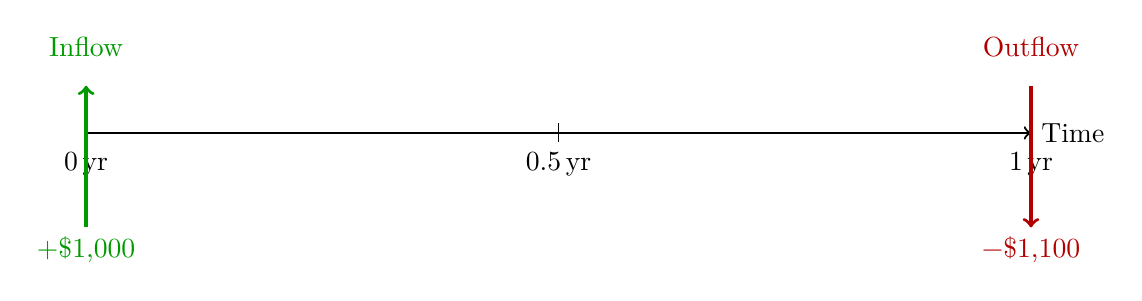
\begin{tikzpicture}[scale=1.2]
% Time axis
\draw[thick,->] (0,0) -- (10,0) node[right] {Time};
\foreach \x/\label in {0/0, 5/0.5, 10/1}
    \draw (\x,0.1) -- (\x,-0.1) node[below] {\label\,yr};

% Cashflow at t=0 (upward = inflow)
\draw[->,green!60!black,very thick] (0,-1) -- (0,0.5);
\node[below,green!60!black] at (0,-1) {+\$1,000};
\node[above,green!60!black] at (0,0.7) {Inflow};

% Cashflow at t=1 (downward = outflow)
\draw[->,red!70!black,very thick] (10,0.5) -- (10,-1);
\node[above,red!70!black] at (10,0.7) {Outflow};
\node[below,red!70!black] at (10,-1) {−\$1,100};
\end{tikzpicture}
\end{figure}

\subsection{3. Visual Timeline with
Arrows}\label{visual-timeline-with-arrows}

\FloatBarrier

\begin{tcolorbox}[enhanced jigsaw, toptitle=1mm, colbacktitle=quarto-callout-tip-color!10!white, opacityback=0, leftrule=.75mm, breakable, colframe=quarto-callout-tip-color-frame, toprule=.15mm, opacitybacktitle=0.6, coltitle=black, bottomrule=.15mm, colback=white, arc=.35mm, titlerule=0mm, rightrule=.15mm, left=2mm, title=\textcolor{quarto-callout-tip-color}{\faLightbulb}\hspace{0.5em}{Reading Timeline Diagrams}, bottomtitle=1mm]

\begin{itemize}
\tightlist
\item
  \textbf{Horizontal axis}: Time progresses left to right
\item
  \textbf{Vertical arrows}:

  \begin{itemize}
  \tightlist
  \item
    {↑ Upward (green)} = Money IN (positive)
  \item
    {↓ Downward (red)} = Money OUT (negative)
  \end{itemize}
\item
  \textbf{Arrow position}: Where it touches the timeline indicates
  \emph{when}
\end{itemize}

\end{tcolorbox}

\section{Multiple Cashflows: Loan Amortization
Example}\label{multiple-cashflows-loan-amortization-example}

Let's see a more realistic scenario: a 3-year loan of \$10,000 with
annual payments.

\subsection{Cashflow Table}\label{cashflow-table}

\begin{longtable}[]{@{}lllll@{}}
\toprule\noalign{}
Time (years) & Payment & Interest & Principal & Outstanding Balance \\
\midrule\noalign{}
\endhead
\bottomrule\noalign{}
\endlastfoot
0 & +10,000 & --- & --- & 10,000 \\
1 & −3,500 & −500 & −3,000 & 7,000 \\
2 & −3,650 & −350 & −3,300 & 3,700 \\
3 & −3,885 & −185 & −3,700 & 0 \\
\end{longtable}

\FloatBarrier

\begin{tcolorbox}[enhanced jigsaw, toptitle=1mm, colbacktitle=quarto-callout-note-color!10!white, opacityback=0, leftrule=.75mm, breakable, colframe=quarto-callout-note-color-frame, toprule=.15mm, opacitybacktitle=0.6, coltitle=black, bottomrule=.15mm, colback=white, arc=.35mm, titlerule=0mm, rightrule=.15mm, left=2mm, title=\textcolor{quarto-callout-note-color}{\faInfo}\hspace{0.5em}{Understanding the Table}, bottomtitle=1mm]

\begin{itemize}
\tightlist
\item
  \textbf{Time 0}: Borrower receives the loan (+\$10,000 inflow)
\item
  \textbf{Each year}: Borrower makes a payment (outflow), which splits
  into:

  \begin{itemize}
  \tightlist
  \item
    \textbf{Interest}: Cost of borrowing (compensation to lender)
  \item
    \textbf{Principal}: Reduction in the debt amount
  \end{itemize}
\item
  \textbf{Outstanding Balance}: What remains to be paid
\end{itemize}

\end{tcolorbox}

\subsection{Timeline Representation}\label{timeline-representation}

\begin{figure}[h]
\centering
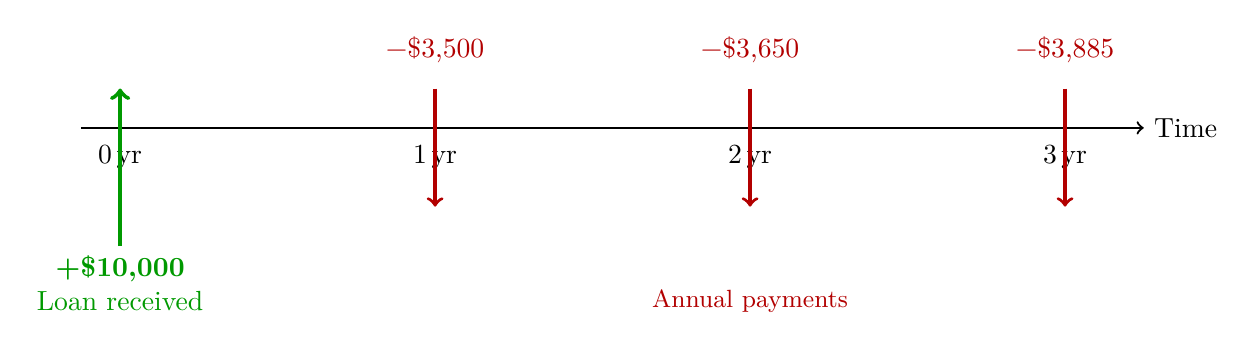
\begin{tikzpicture}[scale=1.0]
% Time axis
\draw[thick,->] (-0.5,0) -- (13,0) node[right] {Time};
\foreach \x/\label in {0/0, 4/1, 8/2, 12/3}
    \draw (\x,0.1) -- (\x,-0.1) node[below] {\label\,yr};

% Initial inflow at t=0
\draw[->,green!60!black,ultra thick] (0,-1.5) -- (0,0.5);
\node[below,green!60!black,font=\bfseries] at (0,-1.5) {+\$10,000};

% Outflows at t=1,2,3
\draw[->,red!70!black,very thick] (4,0.5) -- (4,-1);
\node[above,red!70!black] at (4,0.7) {−\$3,500};

\draw[->,red!70!black,very thick] (8,0.5) -- (8,-1);
\node[above,red!70!black] at (8,0.7) {−\$3,650};

\draw[->,red!70!black,very thick] (12,0.5) -- (12,-1);
\node[above,red!70!black] at (12,0.7) {−\$3,885};

% Labels
\node[green!60!black] at (0,-2.2) {Loan received};
\node[red!70!black,font=\small] at (8,-2.2) {Annual payments};
\end{tikzpicture}
\end{figure}

\FloatBarrier

\section{Investment vs.~Financing
Cashflows}\label{investment-vs.-financing-cashflows}

Two fundamental patterns emerge in financial mathematics:

\subsection{Investment Cashflow
Pattern}\label{investment-cashflow-pattern}

\textbf{Typical structure}: Initial outflow, followed by inflows

\begin{figure}[h]
\centering
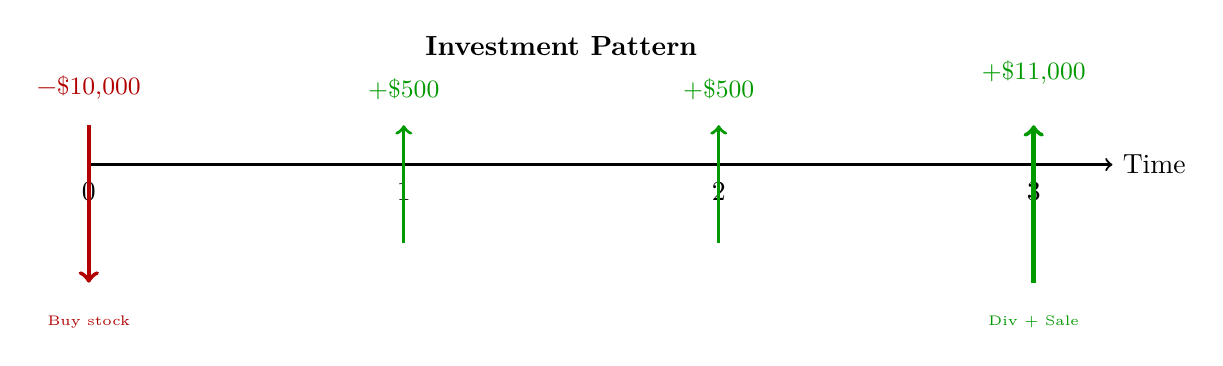
\begin{tikzpicture}[scale=1.0]
% Time axis
\draw[thick,->] (0,0) -- (13,0) node[right] {Time};
\foreach \x/\label in {0/0, 4/1, 8/2, 12/3}
    \draw (\x,0.1) -- (\x,-0.1) node[below] {\label};

% Initial outflow at t=0
\draw[->,red!70!black,ultra thick] (0,0.5) -- (0,-1.5);
\node[above,red!70!black,font=\small] at (0,0.7) {−\$10,000};
\node[below,red!70!black,font=\tiny] at (0,-1.8) {Buy stock};

% Inflows at t=1,2
\foreach \x in {4,8} {
    \draw[->,green!60!black,very thick] (\x,-1) -- (\x,0.5);
    \node[above,green!60!black,font=\small] at (\x,0.7) {+\$500};
}

% Final inflow at t=3
\draw[->,green!60!black,ultra thick] (12,-1.5) -- (12,0.5);
\node[above,green!60!black,font=\small] at (12,0.9) {+\$11,000};
\node[below,green!60!black,font=\tiny] at (12,-1.8) {Div + Sale};

% Label
\node[font=\bfseries] at (6,1.5) {Investment Pattern};
\end{tikzpicture}
\end{figure}

\textbf{Examples}:

\begin{itemize}
\tightlist
\item
  Buying stocks or bonds
\item
  Starting a business
\item
  Purchasing rental property
\end{itemize}

\subsection{Financing Cashflow
Pattern}\label{financing-cashflow-pattern}

\textbf{Typical structure}: Initial inflow, followed by outflows

\begin{figure}[h]
\centering
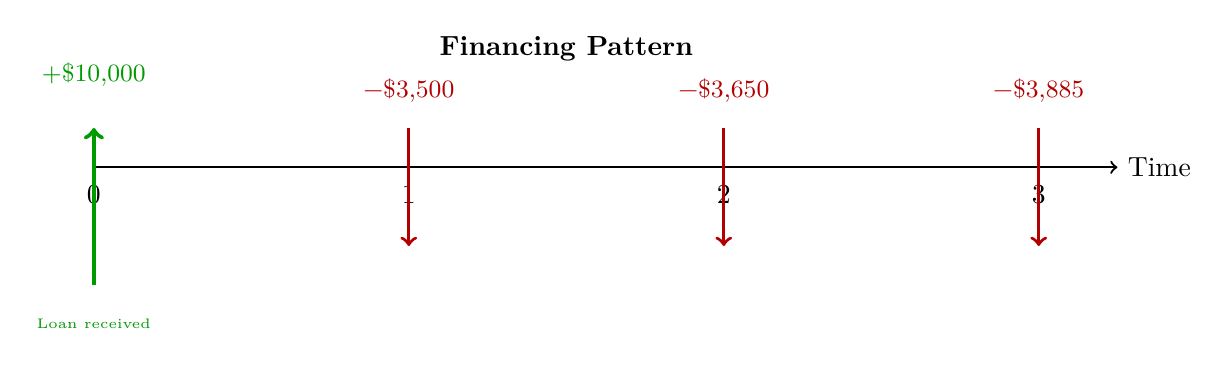
\begin{tikzpicture}[scale=1.0]
% Time axis
\draw[thick,->] (0,0) -- (13,0) node[right] {Time};
\foreach \x/\label in {0/0, 4/1, 8/2, 12/3}
    \draw (\x,0.1) -- (\x,-0.1) node[below] {\label};

% Initial inflow at t=0
\draw[->,green!60!black,ultra thick] (0,-1.5) -- (0,0.5);
\node[above,green!60!black,font=\small] at (0,0.9) {+\$10,000};
\node[below,green!60!black,font=\tiny] at (0,-1.8) {Loan received};

% Outflows at t=1,2,3
\draw[->,red!70!black,very thick] (4,0.5) -- (4,-1);
\node[above,red!70!black,font=\small] at (4,0.7) {−\$3,500};

\draw[->,red!70!black,very thick] (8,0.5) -- (8,-1);
\node[above,red!70!black,font=\small] at (8,0.7) {−\$3,650};

\draw[->,red!70!black,very thick] (12,0.5) -- (12,-1);
\node[above,red!70!black,font=\small] at (12,0.7) {−\$3,885};

% Label
\node[font=\bfseries] at (6,1.5) {Financing Pattern};
\end{tikzpicture}
\end{figure}

\textbf{Examples}:

\begin{itemize}
\tightlist
\item
  Taking a loan
\item
  Issuing bonds (from issuer's perspective)
\item
  Credit card borrowing
\end{itemize}

\begin{tcolorbox}[enhanced jigsaw, toptitle=1mm, colbacktitle=quarto-callout-important-color!10!white, opacityback=0, leftrule=.75mm, breakable, colframe=quarto-callout-important-color-frame, toprule=.15mm, opacitybacktitle=0.6, coltitle=black, bottomrule=.15mm, colback=white, arc=.35mm, titlerule=0mm, rightrule=.15mm, left=2mm, title=\textcolor{quarto-callout-important-color}{\faExclamation}\hspace{0.5em}{Key Insight}, bottomtitle=1mm]

\textbf{Investment} and \textbf{financing} are mirror images of each
other!

\begin{itemize}
\tightlist
\item
  An investor's outflow is the borrower's inflow
\item
  The lender's expected returns = the borrower's cost of capital
\end{itemize}

\end{tcolorbox}

\section{Time Conventions and
Periods}\label{time-conventions-and-periods}

\subsection{Time Measurement}\label{time-measurement}

\begin{tcolorbox}[enhanced jigsaw, toptitle=1mm, colbacktitle=quarto-callout-note-color!10!white, opacityback=0, leftrule=.75mm, breakable, colframe=quarto-callout-note-color-frame, toprule=.15mm, opacitybacktitle=0.6, coltitle=black, bottomrule=.15mm, colback=white, arc=.35mm, titlerule=0mm, rightrule=.15mm, left=2mm, title=\textcolor{quarto-callout-note-color}{\faInfo}\hspace{0.5em}{Definition: Time Index}, bottomtitle=1mm]

We typically denote time by \(t\), measured in \textbf{years} unless
otherwise specified.

\begin{itemize}
\tightlist
\item
  \(t = 0\): Today (present moment)
\item
  \(t = 1\): One year from now
\item
  \(t = 0.5\): Six months from now
\item
  \(t = -1\): One year ago
\end{itemize}

\end{tcolorbox}

\subsection{Period vs.~Point-in-Time}\label{period-vs.-point-in-time}

Be careful to distinguish:

\begin{itemize}
\tightlist
\item
  \textbf{Point in time} (e.g., \(t=2\)): A specific moment
\item
  \textbf{Time period} (e.g., ``year 2''): The interval from \(t=1\) to
  \(t=2\)
\end{itemize}

\textbf{Interest earned in year 2} refers to the interval \([1, 2]\),
but the \textbf{payment at time 2} refers to the instant \(t=2\).

\section{Practical Example: Planning a
Project}\label{practical-example-planning-a-project}

Let's apply these concepts to a realistic business scenario.

\textbf{Scenario}: You're evaluating a software project:

\begin{itemize}
\tightlist
\item
  \textbf{Year 0}: Hire developers, invest \$200,000
\item
  \textbf{Year 1}: Beta launch, invest \$100,000 more
\item
  \textbf{Year 2}: First revenue \$150,000
\item
  \textbf{Year 3}: Mature revenue \$250,000
\end{itemize}

\subsection{Cashflow Table (Your Perspective as
Investor)}\label{cashflow-table-your-perspective-as-investor}

\begin{longtable}[]{@{}lll@{}}
\toprule\noalign{}
Time & Cashflow & Description \\
\midrule\noalign{}
\endhead
\bottomrule\noalign{}
\endlastfoot
0 & −200,000 & Initial development \\
1 & −100,000 & Continued investment \\
2 & +150,000 & First revenue \\
3 & +250,000 & Mature revenue \\
\end{longtable}

\subsection{Net Position Over Time}\label{net-position-over-time}

\begin{longtable}[]{@{}lll@{}}
\toprule\noalign{}
Time & Cashflow & Cumulative Net \\
\midrule\noalign{}
\endhead
\bottomrule\noalign{}
\endlastfoot
0 & −200,000 & −200,000 \\
1 & −100,000 & −300,000 \\
2 & +150,000 & −150,000 \\
3 & +250,000 & +100,000 \\
\end{longtable}

\FloatBarrier

\begin{tcolorbox}[enhanced jigsaw, toptitle=1mm, colbacktitle=quarto-callout-tip-color!10!white, opacityback=0, leftrule=.75mm, breakable, colframe=quarto-callout-tip-color-frame, toprule=.15mm, opacitybacktitle=0.6, coltitle=black, bottomrule=.15mm, colback=white, arc=.35mm, titlerule=0mm, rightrule=.15mm, left=2mm, title=\textcolor{quarto-callout-tip-color}{\faLightbulb}\hspace{0.5em}{Intuition: The Cumulative View}, bottomtitle=1mm]

The \textbf{cumulative net} position shows when you ``break even'' and
start being net positive. Here, you need to wait until after year 3 to
have a positive net position (ignoring time value of money for now).

\end{tcolorbox}

\section{Summary}\label{summary}

Before moving forward, make sure you understand:

✅ \textbf{Cashflows} have amount, timing, and direction\\
✅ \textbf{Sign convention}: Positive = inflow, Negative = outflow\\
✅ \textbf{Perspective matters}: Same transaction looks different to
different parties\\
✅ \textbf{Three representations}: Tables, timelines, and diagrams all
show the same information\\
✅ \textbf{Two patterns}: Investment (− then +) vs.~Financing (+ then −)

\begin{tcolorbox}[enhanced jigsaw, toptitle=1mm, colbacktitle=quarto-callout-warning-color!10!white, opacityback=0, leftrule=.75mm, breakable, colframe=quarto-callout-warning-color-frame, toprule=.15mm, opacitybacktitle=0.6, coltitle=black, bottomrule=.15mm, colback=white, arc=.35mm, titlerule=0mm, rightrule=.15mm, left=2mm, title=\textcolor{quarto-callout-warning-color}{\faExclamationTriangle}\hspace{0.5em}{Common Pitfall}, bottomtitle=1mm]

Don't mix perspectives! If you start from the borrower's viewpoint, stay
consistent. Switching midway through a problem causes sign errors.

\end{tcolorbox}

\begin{tcolorbox}[enhanced jigsaw, toptitle=1mm, colbacktitle=quarto-callout-caution-color!10!white, opacityback=0, leftrule=.75mm, breakable, colframe=quarto-callout-caution-color-frame, toprule=.15mm, opacitybacktitle=0.6, coltitle=black, bottomrule=.15mm, colback=white, arc=.35mm, titlerule=0mm, rightrule=.15mm, left=2mm, title=\textcolor{quarto-callout-caution-color}{\faFire}\hspace{0.5em}{References}, bottomtitle=1mm]

\textbf{Book:} Pearson Corporate Finance 6th Edition, Chapter 4 (The
Time Value of Money), Page 105,
\href{https://cdn.jsdelivr.net/gh/mrbungie/financial_maths@main/resources/books/pearson_corporate_finance_6th.pdf\#page=105}{Direct
Link}

\textbf{Slide:} Financial Mathematics Slides 1-96, Slides 4-23 (Module
1: Basic Notions - Financial transactions, graphical representation,
terminology), Page 4,
\href{https://cdn.jsdelivr.net/gh/mrbungie/financial_maths@main/resources/slideshows/25_09_30_FinancialMathematics_Slides_1_96.pdf\#page=4}{Direct
Link}

\end{tcolorbox}

\begin{center}\rule{0.5\linewidth}{0.5pt}\end{center}

\textbf{Next}: In \href{bonds.qmd}{Chapter 2: Bonds}, we'll apply these
cashflow concepts to understand bond pricing and accrued interest.

\bookmarksetup{startatroot}

\chapter{Bonds}\label{bonds}

\section{Introduction}\label{introduction-1}

Bonds are one of the most important financial instruments. Think of a
bond as a \textbf{formalized loan} with a specific structure: the issuer
borrows money from bondholders and promises regular interest payments
plus return of principal.

\section{What Is a Bond?}\label{what-is-a-bond}

\begin{tcolorbox}[enhanced jigsaw, toptitle=1mm, colbacktitle=quarto-callout-note-color!10!white, opacityback=0, leftrule=.75mm, breakable, colframe=quarto-callout-note-color-frame, toprule=.15mm, opacitybacktitle=0.6, coltitle=black, bottomrule=.15mm, colback=white, arc=.35mm, titlerule=0mm, rightrule=.15mm, left=2mm, title=\textcolor{quarto-callout-note-color}{\faInfo}\hspace{0.5em}{Definition: Bond}, bottomtitle=1mm]

A \textbf{bond} is a debt security with the following components:

\begin{itemize}
\tightlist
\item
  \textbf{Face Value (Par Value)}: The amount to be repaid at maturity
  (typically \$1,000 or \$100)
\item
  \textbf{Coupon Rate}: The annual interest rate applied to face value
\item
  \textbf{Coupon Payment}: Periodic interest payment (usually
  semi-annual or annual)
\item
  \textbf{Maturity Date}: When the face value is repaid
\item
  \textbf{Issue Date}: When the bond is first sold
\end{itemize}

\end{tcolorbox}

\begin{tcolorbox}[enhanced jigsaw, toptitle=1mm, colbacktitle=quarto-callout-tip-color!10!white, opacityback=0, leftrule=.75mm, breakable, colframe=quarto-callout-tip-color-frame, toprule=.15mm, opacitybacktitle=0.6, coltitle=black, bottomrule=.15mm, colback=white, arc=.35mm, titlerule=0mm, rightrule=.15mm, left=2mm, title=\textcolor{quarto-callout-tip-color}{\faLightbulb}\hspace{0.5em}{Intuition: Bond as a Structured Loan}, bottomtitle=1mm]

When you buy a bond:

\begin{itemize}
\tightlist
\item
  You're lending money to the issuer (government, corporation)
\item
  The \textbf{coupon} is your interest income (like a dividend)
\item
  At \textbf{maturity}, you get your principal back
\item
  Unlike stocks, bonds have a \textbf{fixed schedule} of payments
\end{itemize}

\end{tcolorbox}

\section{Simple Bond Example}\label{simple-bond-example}

Let's start with a basic 3-year bond:

\begin{itemize}
\tightlist
\item
  \textbf{Face Value}: \$1,000
\item
  \textbf{Coupon Rate}: 5\% per year
\item
  \textbf{Coupon Frequency}: Annual
\item
  \textbf{Maturity}: 3 years
\end{itemize}

\subsection{Cashflow Table (Bondholder's
Perspective)}\label{cashflow-table-bondholders-perspective}

\begin{longtable}[]{@{}
  >{\raggedright\arraybackslash}p{(\linewidth - 8\tabcolsep) * \real{0.1750}}
  >{\raggedright\arraybackslash}p{(\linewidth - 8\tabcolsep) * \real{0.2000}}
  >{\raggedright\arraybackslash}p{(\linewidth - 8\tabcolsep) * \real{0.2625}}
  >{\raggedright\arraybackslash}p{(\linewidth - 8\tabcolsep) * \real{0.2000}}
  >{\raggedright\arraybackslash}p{(\linewidth - 8\tabcolsep) * \real{0.1625}}@{}}
\toprule\noalign{}
\begin{minipage}[b]{\linewidth}\raggedright
Time (years)
\end{minipage} & \begin{minipage}[b]{\linewidth}\raggedright
Coupon Payment
\end{minipage} & \begin{minipage}[b]{\linewidth}\raggedright
Principal Repayment
\end{minipage} & \begin{minipage}[b]{\linewidth}\raggedright
Total Cashflow
\end{minipage} & \begin{minipage}[b]{\linewidth}\raggedright
Description
\end{minipage} \\
\midrule\noalign{}
\endhead
\bottomrule\noalign{}
\endlastfoot
0 & --- & ---1,000 & −1,000 & Purchase bond \\
1 & +50 & 0 & +50 & First coupon \\
2 & +50 & 0 & +50 & Second coupon \\
3 & +50 & +1,000 & +1,050 & Final coupon + principal \\
\end{longtable}

\textbf{Calculation}: Annual coupon = Face Value × Coupon Rate = \$1,000
× 5\% = \(50\)

\FloatBarrier

\subsection{Timeline Diagram}\label{timeline-diagram-1}

\begin{figure}[h]
\centering
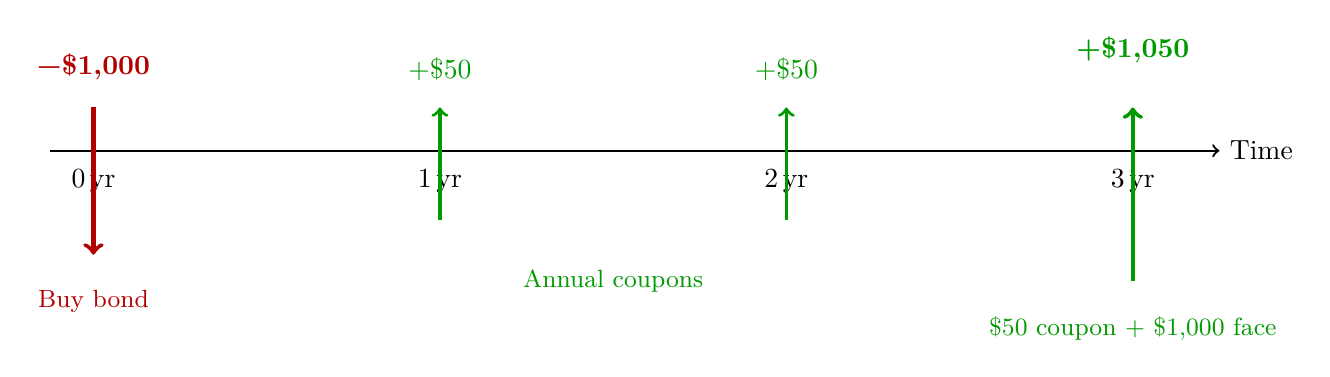
\begin{tikzpicture}[scale=1.1]
% Time axis
\draw[thick,->] (-0.5,0) -- (13,0) node[right] {Time};
\foreach \x/\label in {0/0, 4/1, 8/2, 12/3}
    \draw (\x,0.1) -- (\x,-0.1) node[below] {\label\,yr};

% Purchase at t=0 (outflow)
\draw[->,red!70!black,ultra thick] (0,0.5) -- (0,-1.2);
\node[above,red!70!black,font=\bfseries] at (0,0.7) {−\$1,000};
\node[below,red!70!black,font=\small] at (0,-1.5) {Buy bond};

% Coupons at t=1,2,3 (inflows)
\foreach \x in {4,8} {
    \draw[->,green!60!black,very thick] (\x,-0.8) -- (\x,0.5);
    \node[above,green!60!black] at (\x,0.7) {+\$50};
}

% Final payment at t=3 (coupon + principal)
\draw[->,green!60!black,ultra thick] (12,-1.5) -- (12,0.5);
\node[above,green!60!black,font=\bfseries] at (12,0.9) {+\$1,050};
\node[below,green!60!black,font=\small] at (12,-1.8) {\$50 coupon + \$1,000 face};

% Labels
\node[green!60!black,font=\small] at (6,-1.5) {Annual coupons};
\end{tikzpicture}
\end{figure}

\FloatBarrier

\section{Clean Price vs.~Dirty Price}\label{clean-price-vs.-dirty-price}

When bonds are traded between coupon payment dates, we need to account
for \textbf{accrued interest}.

\begin{tcolorbox}[enhanced jigsaw, toptitle=1mm, colbacktitle=quarto-callout-note-color!10!white, opacityback=0, leftrule=.75mm, breakable, colframe=quarto-callout-note-color-frame, toprule=.15mm, opacitybacktitle=0.6, coltitle=black, bottomrule=.15mm, colback=white, arc=.35mm, titlerule=0mm, rightrule=.15mm, left=2mm, title=\textcolor{quarto-callout-note-color}{\faInfo}\hspace{0.5em}{Definitions}, bottomtitle=1mm]

\textbf{Clean Price (Quoted Price)}: The market price \emph{excluding}
accrued interest. This is what you see quoted.

\textbf{Dirty Price (Invoice Price)}: The actual amount paid = Clean
Price + Accrued Interest

\textbf{Accrued Interest}: Interest earned from the last coupon date to
the settlement date, owed to the seller

\end{tcolorbox}

\subsection{Why Accrued Interest?}\label{why-accrued-interest}

Imagine you buy a bond halfway through a coupon period:

\begin{itemize}
\tightlist
\item
  The seller held the bond for half the period → earned half the coupon
\item
  You'll receive the \emph{full} coupon on the payment date
\item
  \textbf{Fair solution}: You pay the seller for the interest they
  earned but won't receive
\end{itemize}

\begin{tcolorbox}[enhanced jigsaw, toptitle=1mm, colbacktitle=quarto-callout-tip-color!10!white, opacityback=0, leftrule=.75mm, breakable, colframe=quarto-callout-tip-color-frame, toprule=.15mm, opacitybacktitle=0.6, coltitle=black, bottomrule=.15mm, colback=white, arc=.35mm, titlerule=0mm, rightrule=.15mm, left=2mm, title=\textcolor{quarto-callout-tip-color}{\faLightbulb}\hspace{0.5em}{Intuition: ``Rent'' for the Time Period}, bottomtitle=1mm]

Think of accrued interest as rent for the portion of the coupon period
the seller held the bond. They earned that interest; you're compensating
them since you'll collect the full coupon.

\end{tcolorbox}

\section{Visualizing Accrued
Interest}\label{visualizing-accrued-interest}

Let's say you buy a bond 4 months into a 12-month coupon period (4/12 =
1/3 of the period elapsed).

\subsection{Timeline Bar: Elapsed
vs.~Remaining}\label{timeline-bar-elapsed-vs.-remaining}

\begin{figure}[h]
\centering
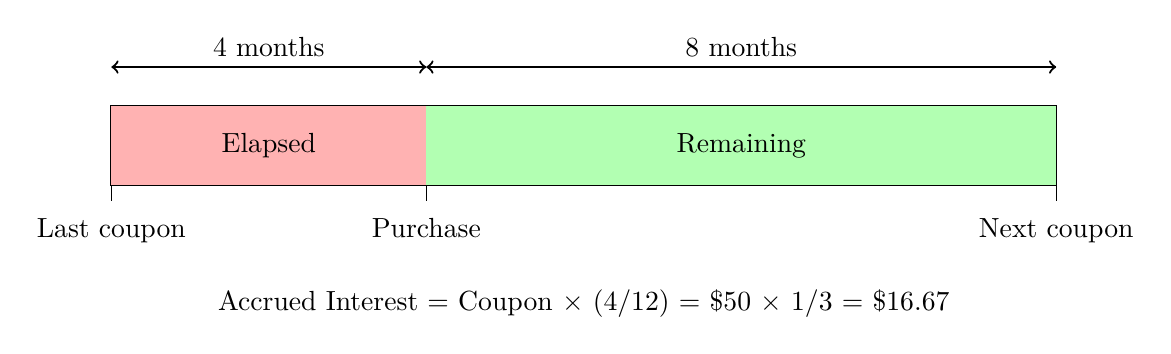
\begin{tikzpicture}
% Full period bar
\draw[thick] (0,0) rectangle (12,1);
\fill[red!30] (0,0) rectangle (4,1);
\fill[green!30] (4,0) rectangle (12,1);

% Labels
\node at (2,0.5) {Elapsed};
\node at (8,0.5) {Remaining};
\node[below] at (0,-0.3) {Last coupon};
\node[below] at (4,-0.3) {Purchase};
\node[below] at (12,-0.3) {Next coupon};

% Time markers
\draw (0,0) -- (0,-0.2);
\draw (4,0) -- (4,-0.2);
\draw (12,0) -- (12,-0.2);

% Arrows
\draw[<->,thick] (0,1.5) -- (4,1.5) node[midway,above] {4 months};
\draw[<->,thick] (4,1.5) -- (12,1.5) node[midway,above] {8 months};

% Accrued interest calculation
\node[align=center] at (6,-1.5) {Accrued Interest = Coupon $\times$ (4/12) = \$50 $\times$ 1/3 = \$16.67};
\end{tikzpicture}
\end{figure}

\subsection{Price Components: Stacked
Boxes}\label{price-components-stacked-boxes}

\begin{figure}[h]
\centering
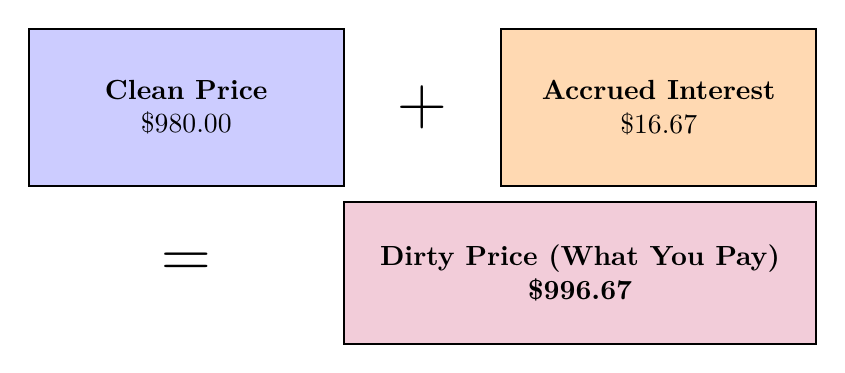
\begin{tikzpicture}
% Clean price box
\draw[thick,fill=blue!20] (0,0) rectangle (4,2);
\node[align=center] at (2,1) {\textbf{Clean Price}\\\$980.00};

% Plus sign
\node[font=\Huge] at (5,1) {+};

% Accrued interest box
\draw[thick,fill=orange!30] (6,0) rectangle (10,2);
\node[align=center] at (8,1) {\textbf{Accrued Interest}\\\$16.67};

% Equals sign
\node[font=\Huge] at (2,-1) {=};

% Dirty price box (wider)
\draw[thick,fill=purple!20] (4,-2) rectangle (10,-0.2);
\node[align=center,font=\bfseries] at (7,-1.1) {Dirty Price (What You Pay)\\\$996.67};
\end{tikzpicture}
\end{figure}

\FloatBarrier

\section{Calculating Accrued
Interest}\label{calculating-accrued-interest}

\begin{tcolorbox}[enhanced jigsaw, toptitle=1mm, colbacktitle=quarto-callout-important-color!10!white, opacityback=0, leftrule=.75mm, breakable, colframe=quarto-callout-important-color-frame, toprule=.15mm, opacitybacktitle=0.6, coltitle=black, bottomrule=.15mm, colback=white, arc=.35mm, titlerule=0mm, rightrule=.15mm, left=2mm, title=\textcolor{quarto-callout-important-color}{\faExclamation}\hspace{0.5em}{Key Formula: Accrued Interest}, bottomtitle=1mm]

\[
\text{Accrued Interest} = \text{Coupon Payment} \times \frac{\text{Days since last coupon}}{\text{Days in coupon period}}
\]

Or equivalently:

\[
AI = C \times \frac{d}{D}
\]

where: - \(C\) = coupon payment - \(d\) = days elapsed since last coupon
- \(D\) = total days in the coupon period

\end{tcolorbox}

\subsection{Day Count Conventions}\label{day-count-conventions}

The ``days'' calculation depends on the \textbf{day count convention}:

\begin{longtable}[]{@{}
  >{\raggedright\arraybackslash}p{(\linewidth - 6\tabcolsep) * \real{0.1905}}
  >{\raggedright\arraybackslash}p{(\linewidth - 6\tabcolsep) * \real{0.2222}}
  >{\raggedright\arraybackslash}p{(\linewidth - 6\tabcolsep) * \real{0.4286}}
  >{\raggedright\arraybackslash}p{(\linewidth - 6\tabcolsep) * \real{0.1587}}@{}}
\toprule\noalign{}
\begin{minipage}[b]{\linewidth}\raggedright
Convention
\end{minipage} & \begin{minipage}[b]{\linewidth}\raggedright
Days in Year
\end{minipage} & \begin{minipage}[b]{\linewidth}\raggedright
Coupon Period Calculation
\end{minipage} & \begin{minipage}[b]{\linewidth}\raggedright
Used For
\end{minipage} \\
\midrule\noalign{}
\endhead
\bottomrule\noalign{}
\endlastfoot
\textbf{ACT/ACT} & Actual (365 or 366) & Actual days in period & US
Treasury bonds \\
\textbf{ACT/360} & 360 & Actual days in period & Corporate bonds,
loans \\
\textbf{30/360} & 360 & Assume 30 days per month & Corporate bonds \\
\end{longtable}

\FloatBarrier

\begin{tcolorbox}[enhanced jigsaw, toptitle=1mm, colbacktitle=quarto-callout-warning-color!10!white, opacityback=0, leftrule=.75mm, breakable, colframe=quarto-callout-warning-color-frame, toprule=.15mm, opacitybacktitle=0.6, coltitle=black, bottomrule=.15mm, colback=white, arc=.35mm, titlerule=0mm, rightrule=.15mm, left=2mm, title=\textcolor{quarto-callout-warning-color}{\faExclamationTriangle}\hspace{0.5em}{Common Pitfall}, bottomtitle=1mm]

Always check which day count convention applies! The same bond can have
different accrued interest depending on the convention used.

\end{tcolorbox}

\subsection{Example Calculation}\label{example-calculation}

\textbf{Given}: - Semi-annual bond (6-month coupons) - Coupon = \$30 -
Last coupon date: January 15 - Purchase date: April 15 - Convention:
ACT/ACT

\textbf{Calculation}: - Days elapsed: Jan 15 → Apr 15 = 90 days (actual
count) - Days in period: Jan 15 → Jul 15 = 181 days (actual) - Accrued
Interest = \$30 × (90/181) = \textbf{\$14.92}

\section{Bond Pricing: Clean vs.~Dirty in
Action}\label{bond-pricing-clean-vs.-dirty-in-action}

Let's see a complete transaction:

\subsection{Market Scenario}\label{market-scenario}

\begin{itemize}
\tightlist
\item
  \textbf{Bond}: 5-year Treasury, 4\% annual coupon, \$1,000 face value
\item
  \textbf{Quoted (Clean) Price}: 98.50 (meaning 98.5\% of face value)
\item
  \textbf{Last coupon date}: 3 months ago
\item
  \textbf{Next coupon}: In 9 months
\item
  \textbf{Convention}: ACT/ACT
\end{itemize}

\subsection{Step 1: Calculate Clean Price in
Dollars}\label{step-1-calculate-clean-price-in-dollars}

\[
\text{Clean Price} = 98.50\% \times \$1,000 = \$985.00
\]

\subsection{Step 2: Calculate Accrued
Interest}\label{step-2-calculate-accrued-interest}

\[
\text{Annual Coupon} = 4\% \times \$1,000 = \$40
\]

\[
\text{Accrued Interest} = \$40 \times \frac{3\text{ months}}{12\text{ months}} = \$40 \times 0.25 = \$10.00
\]

\subsection{Step 3: Calculate Dirty
Price}\label{step-3-calculate-dirty-price}

\[
\text{Dirty Price} = \$985.00 + \$10.00 = \$995.00
\]

\begin{tcolorbox}[enhanced jigsaw, toptitle=1mm, colbacktitle=quarto-callout-tip-color!10!white, opacityback=0, leftrule=.75mm, breakable, colframe=quarto-callout-tip-color-frame, toprule=.15mm, opacitybacktitle=0.6, coltitle=black, bottomrule=.15mm, colback=white, arc=.35mm, titlerule=0mm, rightrule=.15mm, left=2mm, title=\textcolor{quarto-callout-tip-color}{\faLightbulb}\hspace{0.5em}{What You Actually Pay}, bottomtitle=1mm]

You would write a check for \textbf{\$995.00}, even though the bond is
quoted at ``98.50.'' The difference is the seller's compensation for the
3 months of interest they earned.

\end{tcolorbox}

\section{Zero-Coupon Bonds}\label{zero-coupon-bonds}

Not all bonds pay coupons!

\begin{tcolorbox}[enhanced jigsaw, toptitle=1mm, colbacktitle=quarto-callout-note-color!10!white, opacityback=0, leftrule=.75mm, breakable, colframe=quarto-callout-note-color-frame, toprule=.15mm, opacitybacktitle=0.6, coltitle=black, bottomrule=.15mm, colback=white, arc=.35mm, titlerule=0mm, rightrule=.15mm, left=2mm, title=\textcolor{quarto-callout-note-color}{\faInfo}\hspace{0.5em}{Definition: Zero-Coupon Bond}, bottomtitle=1mm]

A \textbf{zero-coupon bond} makes no periodic interest payments.
Instead, it's sold at a discount and redeemed at face value at maturity.

\end{tcolorbox}

\subsection{Example: 5-Year Zero}\label{example-5-year-zero}

\begin{itemize}
\tightlist
\item
  \textbf{Face Value}: \$1,000
\item
  \textbf{Purchase Price}: \$783.53
\item
  \textbf{Maturity}: 5 years
\item
  \textbf{Implied Return}: 5\% per year
\end{itemize}

\subsection{Cashflow Table}\label{cashflow-table-1}

\begin{longtable}[]{@{}lll@{}}
\toprule\noalign{}
Time & Cashflow & Description \\
\midrule\noalign{}
\endhead
\bottomrule\noalign{}
\endlastfoot
0 & −783.53 & Purchase at discount \\
5 & +1,000.00 & Receive face value \\
\end{longtable}

\FloatBarrier

\begin{tcolorbox}[enhanced jigsaw, toptitle=1mm, colbacktitle=quarto-callout-tip-color!10!white, opacityback=0, leftrule=.75mm, breakable, colframe=quarto-callout-tip-color-frame, toprule=.15mm, opacitybacktitle=0.6, coltitle=black, bottomrule=.15mm, colback=white, arc=.35mm, titlerule=0mm, rightrule=.15mm, left=2mm, title=\textcolor{quarto-callout-tip-color}{\faLightbulb}\hspace{0.5em}{Intuition: All Interest at Once}, bottomtitle=1mm]

Instead of receiving small interest payments each year, you receive all
the interest at maturity in the form of the difference between purchase
price and face value (\$1,000 − \$783.53 = \$216.47).

\end{tcolorbox}

\section{Bond Types Summary}\label{bond-types-summary}

\begin{longtable}[]{@{}
  >{\raggedright\arraybackslash}p{(\linewidth - 6\tabcolsep) * \real{0.1579}}
  >{\raggedright\arraybackslash}p{(\linewidth - 6\tabcolsep) * \real{0.2632}}
  >{\raggedright\arraybackslash}p{(\linewidth - 6\tabcolsep) * \real{0.2368}}
  >{\raggedright\arraybackslash}p{(\linewidth - 6\tabcolsep) * \real{0.3421}}@{}}
\toprule\noalign{}
\begin{minipage}[b]{\linewidth}\raggedright
Type
\end{minipage} & \begin{minipage}[b]{\linewidth}\raggedright
Coupons?
\end{minipage} & \begin{minipage}[b]{\linewidth}\raggedright
Example
\end{minipage} & \begin{minipage}[b]{\linewidth}\raggedright
Key Feature
\end{minipage} \\
\midrule\noalign{}
\endhead
\bottomrule\noalign{}
\endlastfoot
\textbf{Fixed-Rate} & Yes, fixed & US Treasury & Predictable income \\
\textbf{Zero-Coupon} & No & STRIPS & Bought at discount \\
\textbf{Floating-Rate} & Yes, variable & Some corporate & Coupon adjusts
with rates \\
\textbf{Callable} & Yes & Municipal bonds & Issuer can repay early \\
\end{longtable}

\FloatBarrier

\section{Practical Insights}\label{practical-insights}

\begin{tcolorbox}[enhanced jigsaw, toptitle=1mm, colbacktitle=quarto-callout-important-color!10!white, opacityback=0, leftrule=.75mm, breakable, colframe=quarto-callout-important-color-frame, toprule=.15mm, opacitybacktitle=0.6, coltitle=black, bottomrule=.15mm, colback=white, arc=.35mm, titlerule=0mm, rightrule=.15mm, left=2mm, title=\textcolor{quarto-callout-important-color}{\faExclamation}\hspace{0.5em}{Why Clean vs.~Dirty Matters}, bottomtitle=1mm]

\textbf{For traders}: Clean price shows the bond's ``true'' value
independent of when you buy it in the coupon cycle.

\textbf{For investors}: Dirty price is what matters for your
cashflow---it's what you actually pay or receive.

\textbf{For comparison}: Clean prices make it easy to compare bonds
without worrying about coupon timing.

\end{tcolorbox}

\section{Summary}\label{summary-1}

✅ \textbf{Bonds} = structured debt with fixed schedules\\
✅ \textbf{Coupons} = periodic interest payments\\
✅ \textbf{Face Value} = principal repaid at maturity\\
✅ \textbf{Clean Price} = quoted price (excludes accrued interest)\\
✅ \textbf{Dirty Price} = actual payment (includes accrued interest)\\
✅ \textbf{Accrued Interest} = seller's compensation for partial
period\\
✅ \textbf{Day Count Conventions} = critical for accurate calculations

\begin{tcolorbox}[enhanced jigsaw, toptitle=1mm, colbacktitle=quarto-callout-caution-color!10!white, opacityback=0, leftrule=.75mm, breakable, colframe=quarto-callout-caution-color-frame, toprule=.15mm, opacitybacktitle=0.6, coltitle=black, bottomrule=.15mm, colback=white, arc=.35mm, titlerule=0mm, rightrule=.15mm, left=2mm, title=\textcolor{quarto-callout-caution-color}{\faFire}\hspace{0.5em}{References}, bottomtitle=1mm]

\textbf{Book:} Pearson Corporate Finance 6th Edition, Chapter 6 (Valuing
Bonds), Page 177,
\href{https://cdn.jsdelivr.net/gh/mrbungie/financial_maths@main/resources/books/pearson_corporate_finance_6th.pdf\#page=177}{Direct
Link}

\textbf{Slide:} Financial Mathematics Slides 1-96, Slides 24-29 (Coupon
bonds, accrued vs dirty price), Page 24,
\href{https://cdn.jsdelivr.net/gh/mrbungie/financial_maths@main/resources/slideshows/25_09_30_FinancialMathematics_Slides_1_96.pdf\#page=24}{Direct
Link}

\end{tcolorbox}

\begin{center}\rule{0.5\linewidth}{0.5pt}\end{center}

\textbf{Next}: In \href{value_function.qmd}{Chapter 3: Value Function},
we'll learn how to value entire cashflow streams over time.

\bookmarksetup{startatroot}

\chapter{Value Function}\label{value-function}

\section{Introduction}\label{introduction-2}

So far, we've learned to describe cashflows as discrete events (money at
specific times). But to truly understand the \textbf{financial state} of
a project or investment at \emph{any} point in time, we need a
continuous view. This is where the \textbf{value function} comes in.

\begin{tcolorbox}[enhanced jigsaw, toptitle=1mm, colbacktitle=quarto-callout-tip-color!10!white, opacityback=0, leftrule=.75mm, breakable, colframe=quarto-callout-tip-color-frame, toprule=.15mm, opacitybacktitle=0.6, coltitle=black, bottomrule=.15mm, colback=white, arc=.35mm, titlerule=0mm, rightrule=.15mm, left=2mm, title=\textcolor{quarto-callout-tip-color}{\faLightbulb}\hspace{0.5em}{Intuition: From Snapshots to a Movie}, bottomtitle=1mm]

\begin{itemize}
\tightlist
\item
  \textbf{Cashflow table}: Snapshots at specific moments
\item
  \textbf{Value function}: A continuous movie showing your financial
  position over time
\end{itemize}

Think of it as tracking your ``net worth from this investment'' at every
instant, not just when money moves.

\end{tcolorbox}

\section{The Core Concept}\label{the-core-concept}

\begin{tcolorbox}[enhanced jigsaw, toptitle=1mm, colbacktitle=quarto-callout-note-color!10!white, opacityback=0, leftrule=.75mm, breakable, colframe=quarto-callout-note-color-frame, toprule=.15mm, opacitybacktitle=0.6, coltitle=black, bottomrule=.15mm, colback=white, arc=.35mm, titlerule=0mm, rightrule=.15mm, left=2mm, title=\textcolor{quarto-callout-note-color}{\faInfo}\hspace{0.5em}{Definition: Value Function}, bottomtitle=1mm]

The \textbf{value function} \(V(t)\) represents the monetary value of a
cashflow stream at time \(t\), accounting for all past and future
cashflows, adjusted for the time value of money.

\[
V(t) = \text{value at time } t \text{ of everything that has happened and will happen}
\]

\end{tcolorbox}

\subsection{\texorpdfstring{Two Perspectives on
\(V(t)\)}{Two Perspectives on V(t)}}\label{two-perspectives-on-vt}

\begin{enumerate}
\def\labelenumi{\arabic{enumi}.}
\tightlist
\item
  \textbf{Backward-looking}: What happened before \(t\), accumulated to
  time \(t\)
\item
  \textbf{Forward-looking}: What will happen after \(t\), discounted to
  time \(t\)
\end{enumerate}

\section{Simple Example: Building
Intuition}\label{simple-example-building-intuition}

Let's start with a simple 2-period investment:

\begin{itemize}
\tightlist
\item
  \textbf{t = 0}: Invest \$100 (outflow)
\item
  \textbf{t = 1}: Receive \$50 (inflow)
\item
  \textbf{t = 2}: Receive \$60 (inflow)
\item
  \textbf{Interest rate}: 5\% per period
\end{itemize}

\subsection{What Is the Value
Function?}\label{what-is-the-value-function}

Let's calculate \(V(t)\) at different points:

\subsubsection{\texorpdfstring{\(V(0)\): Value at the
Start}{V(0): Value at the Start}}\label{v0-value-at-the-start}

At \(t=0\), we can compute value by discounting all future cashflows:

\[
V(0) = -100 + \frac{50}{1.05} + \frac{60}{(1.05)^2} = -100 + 47.62 + 54.42 = 2.04
\]

\textbf{Interpretation}: At the moment of investment, this project is
worth \(2.04\) (it's a good deal---positive NPV!).

\subsubsection{\texorpdfstring{\(V(1)\): Value After One
Period}{V(1): Value After One Period}}\label{v1-value-after-one-period}

At \(t=1\), we've invested \$100 and earned 5\% interest for one year,
plus we receive the \(50\) cashflow:

\[
V(1) = -100 \times 1.05 + 50 = -105 + 50 = -55
\]

But we still have the future \$60 coming:

\[
V(1) = -55 + \frac{60}{1.05} = -55 + 57.14 = 2.14
\]

\textbf{Interpretation}: At \(t=1\), accounting for what's happened and
what's coming, we're worth \(2.14\).

\subsubsection{\texorpdfstring{\(V(2)\): Value at the
End}{V(2): Value at the End}}\label{v2-value-at-the-end}

\[
V(2) = (-100 \times 1.05 + 50) \times 1.05 + 60 = -55 \times 1.05 + 60 = -57.75 + 60 = 2.25
\]

\textbf{Interpretation}: At the end, all cashflows have been realized
and accumulated to \(t=2\).

\subsection{Value Function Graph}\label{value-function-graph}

\begin{figure}[h]
\centering
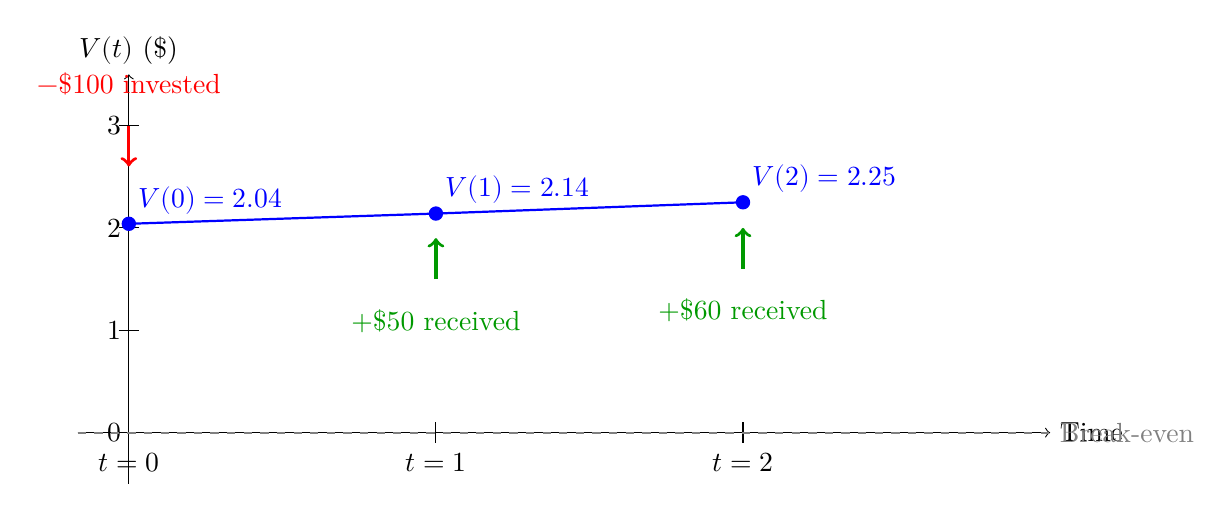
\begin{tikzpicture}[scale=1.3]
% Axes
\draw[->] (-0.5,0) -- (9,0) node[right] {Time};
\draw[->] (0,-0.5) -- (0,3.5) node[above] {$V(t)$ (\$)};

% Y-axis labels
\foreach \y/\label in {0/0, 1/1, 2/2, 3/3}
    \draw (-0.1,\y) -- (0.1,\y) node[left=3pt] {\label};

% Time labels
\foreach \x/\label in {0/0, 3/1, 6/2}
    \draw (\x,0.1) -- (\x,-0.1) node[below] {$t=\label$};

% Value function (smooth curve through calculated points)
% All values are around 2, staying positive throughout
\draw[thick,blue] (0,2.04) -- (3,2.14) -- (6,2.25);

% Value points
\fill[blue] (0,2.04) circle (2pt) node[above right] {$V(0)=2.04$};
\fill[blue] (3,2.14) circle (2pt) node[above right] {$V(1)=2.14$};
\fill[blue] (6,2.25) circle (2pt) node[above right] {$V(2)=2.25$};

% Cashflow arrows (showing direction only, positioned away from line)
\draw[->,red,very thick] (0,3) -- (0,2.6);
\node[above,red] at (0,3.2) {−\$100 invested};

\draw[->,green!60!black,very thick] (3,1.5) -- (3,1.9);
\node[below,green!60!black] at (3,1.3) {+\$50 received};

\draw[->,green!60!black,very thick] (6,1.6) -- (6,2.0);
\node[below,green!60!black] at (6,1.4) {+\$60 received};

% Zero line
\draw[dashed,gray,thick] (-0.5,0) -- (9,0);
\node[right,gray] at (9,0) {Break-even};
\end{tikzpicture}
\end{figure}

\FloatBarrier

\begin{tcolorbox}[enhanced jigsaw, toptitle=1mm, colbacktitle=quarto-callout-tip-color!10!white, opacityback=0, leftrule=.75mm, breakable, colframe=quarto-callout-tip-color-frame, toprule=.15mm, opacitybacktitle=0.6, coltitle=black, bottomrule=.15mm, colback=white, arc=.35mm, titlerule=0mm, rightrule=.15mm, left=2mm, title=\textcolor{quarto-callout-tip-color}{\faLightbulb}\hspace{0.5em}{Reading the Graph}, bottomtitle=1mm]

\begin{itemize}
\tightlist
\item
  \textbf{The value function stays POSITIVE throughout} --- this is a
  good project (NPV \textgreater{} 0)!
\item
  \textbf{It increases slightly over time} from \$2.04 → \$2.14 → \$2.25
  (about 5\% growth)
\item
  The \textbf{height} at any point shows the NPV evaluated at that
  moment in time
\item
  Even though we invest \$100 upfront, the discounted future cashflows
  make the project worthwhile
\item
  The small increase reflects the 5\% interest rate compounding the NPV
  forward
\end{itemize}

\end{tcolorbox}

\section{The Value Function Formula}\label{the-value-function-formula}

\begin{tcolorbox}[enhanced jigsaw, toptitle=1mm, colbacktitle=quarto-callout-important-color!10!white, opacityback=0, leftrule=.75mm, breakable, colframe=quarto-callout-important-color-frame, toprule=.15mm, opacitybacktitle=0.6, coltitle=black, bottomrule=.15mm, colback=white, arc=.35mm, titlerule=0mm, rightrule=.15mm, left=2mm, title=\textcolor{quarto-callout-important-color}{\faExclamation}\hspace{0.5em}{Key Formula: Value Function}, bottomtitle=1mm]

For a cashflow stream with payments \(C_0, C_1, ..., C_n\) at times
\(t_0, t_1, ..., t_n\):

\[
V(t) = \sum_{t_i \leq t} C_i \cdot (1+i)^{t-t_i} + \sum_{t_j > t} \frac{C_j}{(1+i)^{t_j - t}}
\]

Where: - First sum: Past cashflows accumulated forward to time \(t\) -
Second sum: Future cashflows discounted back to time \(t\) - \(i\) =
interest rate per period

\end{tcolorbox}

\textbf{In words}: \textgreater{} Value at time \(t\) = (Everything
before \(t\), grown with interest) + (Everything after \(t\),
discounted)

\section{Multi-Period Decomposition}\label{multi-period-decomposition}

Let's see how \(V(t)\) evolves period by period for a more complex
example.

\subsection{Example: 4-Year Investment}\label{example-4-year-investment}

\textbf{Cashflows}:

\begin{itemize}
\tightlist
\item
  \(t=0\): −\$1,000
\item
  \(t=1\): +\$200
\item
  \(t=2\): +\$300
\item
  \(t=3\): +\$400
\item
  \(t=4\): +\$500
\end{itemize}

\textbf{Interest rate}: 8\% per year

\subsection{Step-by-Step Accumulation}\label{step-by-step-accumulation}

\begin{longtable}[]{@{}
  >{\raggedright\arraybackslash}p{(\linewidth - 8\tabcolsep) * \real{0.1159}}
  >{\raggedright\arraybackslash}p{(\linewidth - 8\tabcolsep) * \real{0.2464}}
  >{\raggedright\arraybackslash}p{(\linewidth - 8\tabcolsep) * \real{0.2464}}
  >{\raggedright\arraybackslash}p{(\linewidth - 8\tabcolsep) * \real{0.1449}}
  >{\raggedright\arraybackslash}p{(\linewidth - 8\tabcolsep) * \real{0.2464}}@{}}
\toprule\noalign{}
\begin{minipage}[b]{\linewidth}\raggedright
Period
\end{minipage} & \begin{minipage}[b]{\linewidth}\raggedright
Opening Balance
\end{minipage} & \begin{minipage}[b]{\linewidth}\raggedright
Interest Earned
\end{minipage} & \begin{minipage}[b]{\linewidth}\raggedright
Cashflow
\end{minipage} & \begin{minipage}[b]{\linewidth}\raggedright
Closing Balance
\end{minipage} \\
\midrule\noalign{}
\endhead
\bottomrule\noalign{}
\endlastfoot
0 → 1 & −1,000 & −80 & +200 & −880 \\
1 → 2 & −880 & −70.40 & +300 & −650.40 \\
2 → 3 & −650.40 & −52.03 & +400 & −302.43 \\
3 → 4 & −302.43 & −24.19 & +500 & +173.38 \\
\end{longtable}

\FloatBarrier

\textbf{Interpretation}:

\begin{itemize}
\tightlist
\item
  We're ``in the hole'' (negative) through year 3
\item
  Interest accumulates on our negative balance (making it more negative)
\item
  Finally, by year 4, we're positive: \textbf{+\$173.38}
\end{itemize}

\subsection{Cumulative Cashflow Graph}\label{cumulative-cashflow-graph}

\begin{figure}[h]
\centering
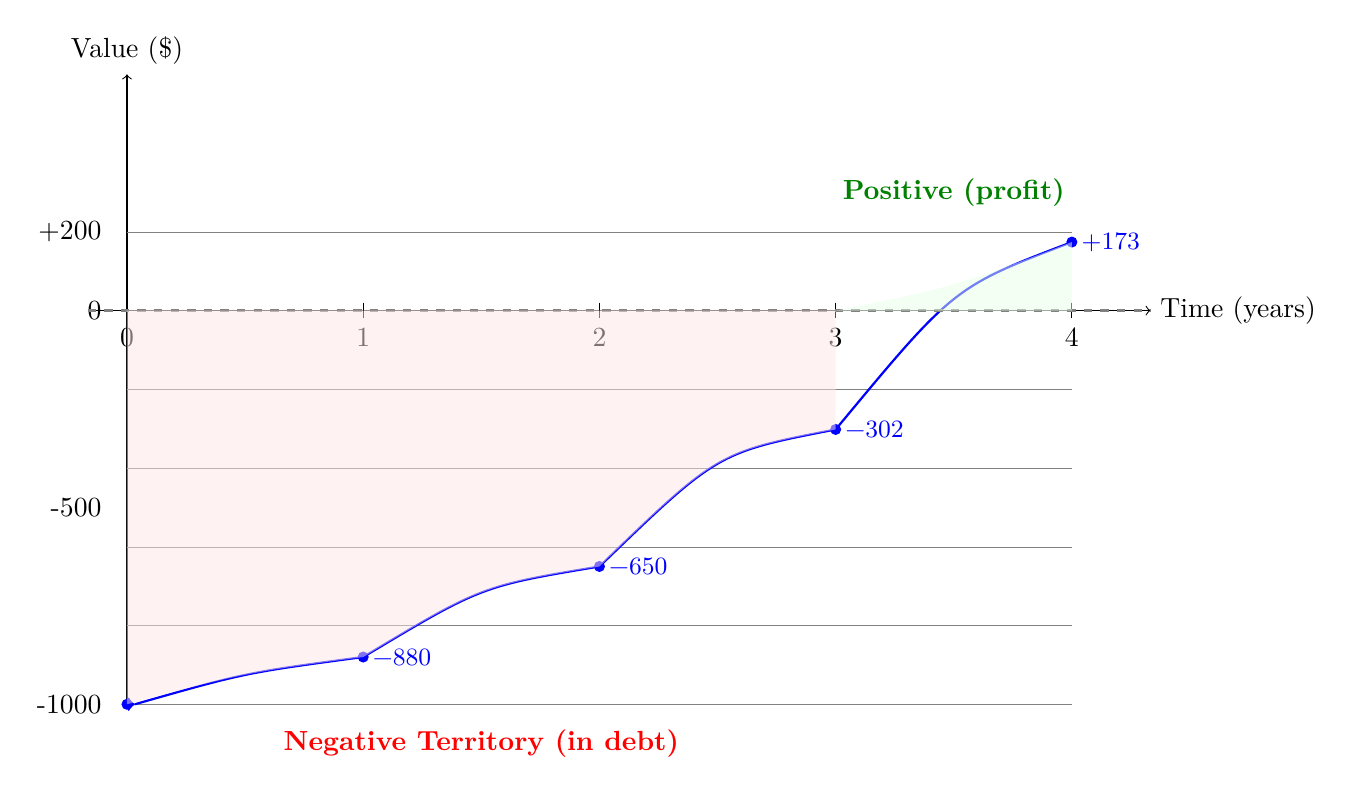
\begin{tikzpicture}[scale=1.0]
% Axes
\draw[->] (-0.5,0) -- (13,0) node[right] {Time (years)};
\draw[->] (0,-5) -- (0,3) node[above] {Value (\$)};

% Grid lines
\foreach \y in {-1000,-800,-600,-400,-200,0,200}
    \draw[gray,very thin] (0,\y/200) -- (12,\y/200);

% Y-axis labels
\foreach \y/\label in {-1000/-1000,-500/-500,0/0,200/+200}
    \node[left] at (-0.2,\y/200) {\label};

% Time markers
\foreach \x/\label in {0/0, 3/1, 6/2, 9/3, 12/4}
    \draw (\x,0.1) -- (\x,-0.1) node[below] {\label};

% Value function (staircase with smooth curves for interest periods)
\draw[thick,blue,->] (0,-5) -- (0.1,-5);
\draw[thick,blue] (0.1,-5) .. controls (1.5,-4.6) .. (3,-4.4);
\draw[thick,blue] (3,-4.4) .. controls (4.5,-3.5) .. (6,-3.25);
\draw[thick,blue] (6,-3.25) .. controls (7.5,-1.8) .. (9,-1.51);
\draw[thick,blue] (9,-1.51) .. controls (10.5,0.3) .. (12,0.87);

% Value points
\fill[blue] (0,-5) circle (2pt);
\fill[blue] (3,-4.4) circle (2pt) node[right,font=\small] {−880};
\fill[blue] (6,-3.25) circle (2pt) node[right,font=\small] {−650};
\fill[blue] (9,-1.51) circle (2pt) node[right,font=\small] {−302};
\fill[blue] (12,0.87) circle (2pt) node[right,font=\small] {+173};

% Zero reference line
\draw[dashed,thick,gray] (-0.5,0) -- (13,0);

% Shading
\fill[red!10,opacity=0.5] (0,0) -- (0,-5) .. controls (1.5,-4.6) .. (3,-4.4) .. controls (4.5,-3.5) .. (6,-3.25) .. controls (7.5,-1.8) .. (9,-1.51) -- (9,0) -- cycle;
\fill[green!10,opacity=0.5] (9,0) .. controls (10.5,0.3) .. (12,0.87) -- (12,0) -- cycle;

% Labels
\node[red,font=\bfseries] at (4.5,-5.5) {Negative Territory (in debt)};
\node[green!50!black,font=\bfseries] at (10.5,1.5) {Positive (profit)};
\end{tikzpicture}
\end{figure}

\FloatBarrier

\begin{tcolorbox}[enhanced jigsaw, toptitle=1mm, colbacktitle=quarto-callout-tip-color!10!white, opacityback=0, leftrule=.75mm, breakable, colframe=quarto-callout-tip-color-frame, toprule=.15mm, opacitybacktitle=0.6, coltitle=black, bottomrule=.15mm, colback=white, arc=.35mm, titlerule=0mm, rightrule=.15mm, left=2mm, title=\textcolor{quarto-callout-tip-color}{\faLightbulb}\hspace{0.5em}{The ``Smoothed Story'' Interpretation}, bottomtitle=1mm]

The value function \(V(t)\) tells a \textbf{smoothed story}:

\begin{itemize}
\tightlist
\item
  Not just ``when does money move?'' (discrete cashflows)
\item
  But ``what is my financial state at every moment?'' (continuous value)
\item
  It accounts for \textbf{interest accumulation} between cashflows
\item
  The curves between jumps show interest working on your balance
\end{itemize}

\end{tcolorbox}

\section{Net Present Value (NPV)}\label{net-present-value-npv}

The value at time zero, \(V(0)\), has a special name:

\begin{tcolorbox}[enhanced jigsaw, toptitle=1mm, colbacktitle=quarto-callout-note-color!10!white, opacityback=0, leftrule=.75mm, breakable, colframe=quarto-callout-note-color-frame, toprule=.15mm, opacitybacktitle=0.6, coltitle=black, bottomrule=.15mm, colback=white, arc=.35mm, titlerule=0mm, rightrule=.15mm, left=2mm, title=\textcolor{quarto-callout-note-color}{\faInfo}\hspace{0.5em}{Definition: Net Present Value}, bottomtitle=1mm]

The \textbf{Net Present Value (NPV)} is the value function evaluated at
\(t=0\):

\[
\text{NPV} = V(0) = \sum_{i=0}^{n} \frac{C_i}{(1+r)^{t_i}}
\]

It represents the ``today value'' of the entire cashflow stream.

\end{tcolorbox}

\subsection{Decision Rule}\label{decision-rule}

\begin{tcolorbox}[enhanced jigsaw, toptitle=1mm, colbacktitle=quarto-callout-important-color!10!white, opacityback=0, leftrule=.75mm, breakable, colframe=quarto-callout-important-color-frame, toprule=.15mm, opacitybacktitle=0.6, coltitle=black, bottomrule=.15mm, colback=white, arc=.35mm, titlerule=0mm, rightrule=.15mm, left=2mm, title=\textcolor{quarto-callout-important-color}{\faExclamation}\hspace{0.5em}{NPV Decision Rule}, bottomtitle=1mm]

\begin{itemize}
\tightlist
\item
  \textbf{NPV \textgreater{} 0}: Project adds value → \textbf{Accept}
\item
  \textbf{NPV = 0}: Project is break-even → \textbf{Indifferent}
\item
  \textbf{NPV \textless{} 0}: Project destroys value → \textbf{Reject}
\end{itemize}

\end{tcolorbox}

\subsection{Example: Should We Accept This
Investment?}\label{example-should-we-accept-this-investment}

\textbf{Investment opportunity}:

\begin{itemize}
\tightlist
\item
  Initial cost: \$5,000
\item
  Year 1 return: \$2,000
\item
  Year 2 return: \$2,500
\item
  Year 3 return: \$1,800
\item
  Discount rate: 10\%
\end{itemize}

\textbf{Calculate NPV}: \[
\begin{aligned}
\text{NPV} &= -5000 + \frac{2000}{1.10} + \frac{2500}{1.10^2} + \frac{1800}{1.10^3} \\
&= -5000 + 1818.18 + 2066.12 + 1352.42 \\
&= 236.72
\end{aligned}
\]

\textbf{Decision}: \textbf{Accept!} NPV = \(236.72\) \textgreater{} 0,
so the project adds value.

\section{Value Function Properties}\label{value-function-properties}

\subsection{Property 1: Additivity}\label{property-1-additivity}

If you have two independent cashflow streams \(A\) and \(B\):

\[
V_{A+B}(t) = V_A(t) + V_B(t)
\]

You can value them separately and add the results.

\subsection{Property 2: Time
Consistency}\label{property-2-time-consistency}

The value function satisfies:

\[
V(t_2) = V(t_1) \cdot (1+i)^{t_2-t_1} + \sum_{t_1 < t_i \leq t_2} C_i \cdot (1+i)^{t_2-t_i}
\]

\textbf{Interpretation}: Value at \(t_2\) = (Value at \(t_1\) grown with
interest) + (Cashflows in between, accumulated)

\subsection{Property 3: Boundary
Conditions}\label{property-3-boundary-conditions}

\begin{itemize}
\tightlist
\item
  \textbf{At start}: \(V(0)\) = NPV
\item
  \textbf{At end}: \(V(T)\) = all cashflows accumulated to final time
\end{itemize}

\section{Practical Applications}\label{practical-applications}

\subsection{1. Project Monitoring}\label{project-monitoring}

Track \(V(t)\) over time to see if your project is on track:

\begin{figure}[h]
\centering
\begin{tikzpicture}[scale=1.0]
% Axes
\draw[->] (0,0) -- (10,0) node[right] {Time};
\draw[->] (0,-2) -- (0,3) node[above] {Value};

% Planned trajectory
\draw[thick,blue,dashed] (0,0.5) -- (2,-0.5) -- (4,0.2) -- (6,1) -- (8,1.6) -- (10,2);
\node[blue] at (10,2.5) {Planned $V(t)$};

% Actual trajectory
\draw[thick,red] (0,0.5) -- (2,-0.3) -- (4,0.4) -- (6,1.2) -- (8,1.9);
\node[red] at (8,2.5) {Actual $V(t)$};

% Current time
\draw[thick,dashed] (8,-2) -- (8,3);
\node[below] at (8,-2) {Today};

% Annotation
\node[green!50!black,font=\small] at (7,1.5) {Ahead of plan! ✓};
\end{tikzpicture}
\end{figure}

\FloatBarrier

If actual \(V(t)\) \textgreater{} planned \(V(t)\), you're ahead of
schedule!

\subsection{2. Comparing Investments}\label{comparing-investments}

Two projects with different cashflow patterns:

\begin{longtable}[]{@{}lll@{}}
\toprule\noalign{}
Time & Project A & Project B \\
\midrule\noalign{}
\endhead
\bottomrule\noalign{}
\endlastfoot
0 & −1,000 & −1,000 \\
1 & +1,200 & 0 \\
2 & 0 & +1,300 \\
\end{longtable}

\textbf{At 10\% discount rate}: -
\(\text{NPV}_A = -1000 + 1200/1.10 = 90.91\) -
\(\text{NPV}_B = -1000 + 1300/1.10^2 = 74.38\)

\textbf{Conclusion}: Project A is better (higher NPV).

\section{Summary}\label{summary-2}

✅ \textbf{Value function} \(V(t)\) = financial position at any time
\(t\)\\
✅ \textbf{Combines} past (accumulated) and future (discounted)
cashflows\\
✅ \textbf{NPV} = \(V(0)\) = value at the start\\
✅ \textbf{Decision rule}: Accept if NPV \textgreater{} 0\\
✅ \textbf{Tells a story}: Smoothed continuous view of wealth over
time\\
✅ \textbf{Practical use}: Monitor projects, compare investments

\begin{tcolorbox}[enhanced jigsaw, toptitle=1mm, colbacktitle=quarto-callout-important-color!10!white, opacityback=0, leftrule=.75mm, breakable, colframe=quarto-callout-important-color-frame, toprule=.15mm, opacitybacktitle=0.6, coltitle=black, bottomrule=.15mm, colback=white, arc=.35mm, titlerule=0mm, rightrule=.15mm, left=2mm, title=\textcolor{quarto-callout-important-color}{\faExclamation}\hspace{0.5em}{Key Insight}, bottomtitle=1mm]

The value function transforms \textbf{discrete cashflows} (jumps) into a
\textbf{continuous financial narrative} (smooth story). It's the ``bank
account balance'' of the investment at every moment.

\end{tcolorbox}

\begin{tcolorbox}[enhanced jigsaw, toptitle=1mm, colbacktitle=quarto-callout-caution-color!10!white, opacityback=0, leftrule=.75mm, breakable, colframe=quarto-callout-caution-color-frame, toprule=.15mm, opacitybacktitle=0.6, coltitle=black, bottomrule=.15mm, colback=white, arc=.35mm, titlerule=0mm, rightrule=.15mm, left=2mm, title=\textcolor{quarto-callout-caution-color}{\faFire}\hspace{0.5em}{References}, bottomtitle=1mm]

\textbf{Book:} Pearson Corporate Finance 6th Edition, Chapter 3 (Present
Value and NPV Decision Rule), Page 74,
\href{https://cdn.jsdelivr.net/gh/mrbungie/financial_maths@main/resources/books/pearson_corporate_finance_6th.pdf\#page=74}{Direct
Link}

\textbf{Slide:} Financial Mathematics Slides 1-96, Slides 33-36 (Value
function definition, properties, examples), Page 33,
\href{https://cdn.jsdelivr.net/gh/mrbungie/financial_maths@main/resources/slideshows/25_09_30_FinancialMathematics_Slides_1_96.pdf\#page=33}{Direct
Link}

\end{tcolorbox}

\begin{center}\rule{0.5\linewidth}{0.5pt}\end{center}

\textbf{Next}: In \href{interest_rates.qmd}{Chapter 4: Interest \&
Discount Rates}, we'll dive deep into how interest rates drive the time
value of money.

\bookmarksetup{startatroot}

\chapter{Interest \& Discount Rates}\label{interest-discount-rates}

\section{Introduction}\label{introduction-3}

Interest rates are the \textbf{engine} of financial mathematics. They
answer the fundamental question: \emph{``What is the price of time?''}
In this chapter, we'll explore how interest rates work, how they relate
to discount factors, and how they transform money across time.

\section{The Time Value of Money}\label{the-time-value-of-money}

\begin{tcolorbox}[enhanced jigsaw, toptitle=1mm, colbacktitle=quarto-callout-note-color!10!white, opacityback=0, leftrule=.75mm, breakable, colframe=quarto-callout-note-color-frame, toprule=.15mm, opacitybacktitle=0.6, coltitle=black, bottomrule=.15mm, colback=white, arc=.35mm, titlerule=0mm, rightrule=.15mm, left=2mm, title=\textcolor{quarto-callout-note-color}{\faInfo}\hspace{0.5em}{Core Principle: Time Value of Money}, bottomtitle=1mm]

\textbf{A dollar today is worth more than a dollar tomorrow.}

Why? Three main reasons:

\begin{enumerate}
\def\labelenumi{\arabic{enumi}.}
\tightlist
\item
  \textbf{Opportunity cost}: Today's dollar can be invested to earn
  returns
\item
  \textbf{Inflation}: Future dollars have less purchasing power
\item
  \textbf{Risk}: Future payments are uncertain
\end{enumerate}

\end{tcolorbox}

Interest rates \textbf{quantify} this time value: they tell us precisely
\emph{how much more} a dollar today is worth compared to a dollar later.

\section{Two Directions: Accumulation
vs.~Discount}\label{two-directions-accumulation-vs.-discount}

Think of interest rates as a \textbf{bidirectional lens} for viewing
money across time:

\begin{tcolorbox}[enhanced jigsaw, toptitle=1mm, colbacktitle=quarto-callout-tip-color!10!white, opacityback=0, leftrule=.75mm, breakable, colframe=quarto-callout-tip-color-frame, toprule=.15mm, opacitybacktitle=0.6, coltitle=black, bottomrule=.15mm, colback=white, arc=.35mm, titlerule=0mm, rightrule=.15mm, left=2mm, title=\textcolor{quarto-callout-tip-color}{\faLightbulb}\hspace{0.5em}{The ``Money Lens'' Analogy}, bottomtitle=1mm]

\textbf{🔭 Accumulation = Telescope (Forward View)}\\
Looking into the future: \emph{``If I invest \$100 today, how much will
I have later?''}\\
Answer: \textbf{More} (money grows)

\textbf{🔬 Discount = Microscope (Backward View)}\\
Looking back to present: \emph{``If I need \$100 in the future, how much
should I set aside today?''}\\
Answer: \textbf{Less} (future dollars are worth less today)

\end{tcolorbox}

\subsection{Visual: Mirrored Diagrams}\label{visual-mirrored-diagrams}

\begin{figure}[h]
\centering
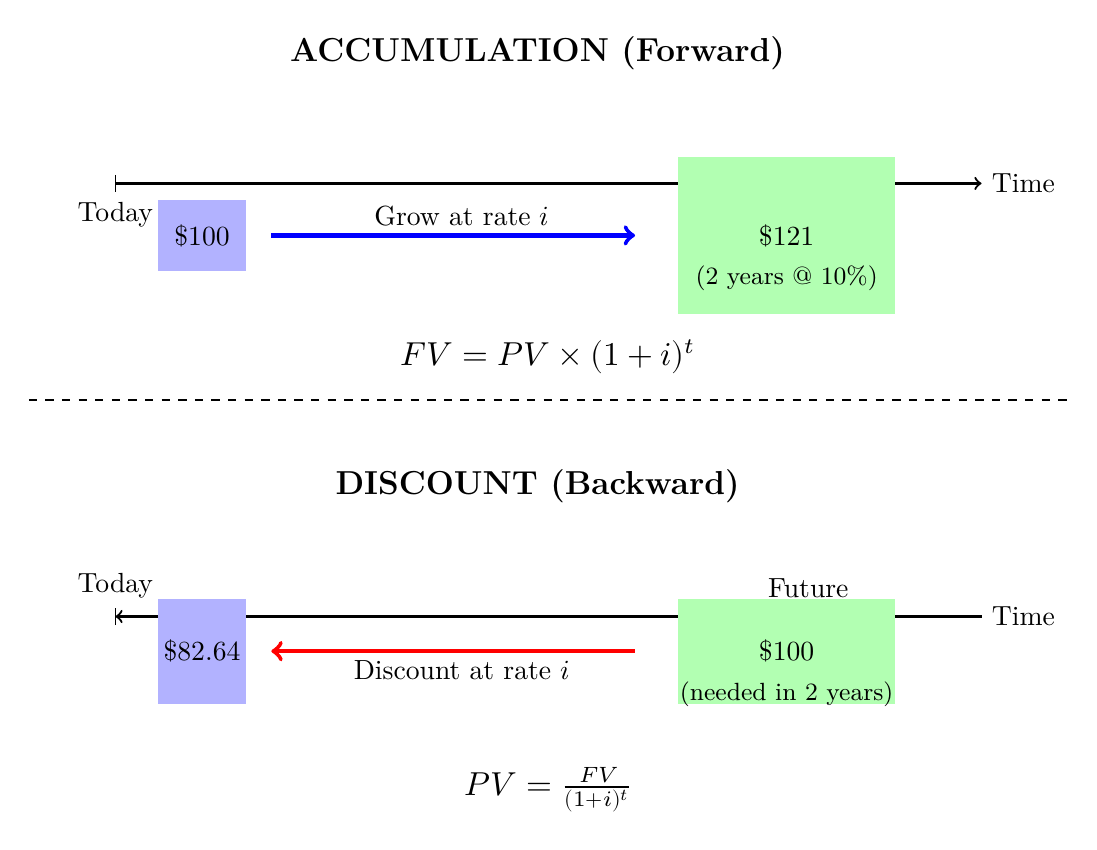
\begin{tikzpicture}[scale=1.1]
% ACCUMULATION (top half)
\node[font=\large\bfseries] at (5,4) {ACCUMULATION (Forward) 🔭};

% Time axis
\draw[thick,->] (0,2.5) -- (10,2.5) node[right] {Time};
\draw (0,2.6) -- (0,2.4) node[below] {Today};
\draw (8,2.6) -- (8,2.4) node[below] {Future};

% Amount growth
\filldraw[blue!30] (0.5,1.5) rectangle (1.5,2.3);
\node at (1,1.9) {\$100};
\draw[->,ultra thick,blue] (1.8,1.9) -- (6,1.9);
\node[above] at (4,1.9) {Grow at rate $i$};
\filldraw[green!30] (6.5,1) rectangle (9,2.8);
\node at (7.75,1.9) {\$121};
\node[font=\small] at (7.75,1.4) {(2 years @ 10\%)};

% Formula
\node[font=\large] at (5,0.5) {$FV = PV \times (1+i)^t$};

% Separator
\draw[thick,dashed] (-1,0) -- (11,0);

% DISCOUNT (bottom half)
\node[font=\large\bfseries] at (5,-1) {DISCOUNT (Backward) 🔬};

% Time axis (reversed direction emphasis)
\draw[thick,<-] (0,-2.5) -- (10,-2.5) node[right] {Time};
\draw (0,-2.6) -- (0,-2.4) node[above] {Today};
\draw (8,-2.6) -- (8,-2.4) node[above] {Future};

% Amount shrinkage
\filldraw[blue!30] (0.5,-2.3) rectangle (1.5,-3.5);
\node at (1,-2.9) {\$82.64};
\draw[<-,ultra thick,red] (1.8,-2.9) -- (6,-2.9);
\node[below] at (4,-2.9) {Discount at rate $i$};
\filldraw[green!30] (6.5,-2.3) rectangle (9,-3.5);
\node at (7.75,-2.9) {\$100};
\node[font=\small] at (7.75,-3.4) {(needed in 2 years)};

% Formula
\node[font=\large] at (5,-4.5) {$PV = \frac{FV}{(1+i)^t}$};
\end{tikzpicture}
\end{figure}

\section{Accumulation: Growing Money
Forward}\label{accumulation-growing-money-forward}

\begin{tcolorbox}[enhanced jigsaw, toptitle=1mm, colbacktitle=quarto-callout-note-color!10!white, opacityback=0, leftrule=.75mm, breakable, colframe=quarto-callout-note-color-frame, toprule=.15mm, opacitybacktitle=0.6, coltitle=black, bottomrule=.15mm, colback=white, arc=.35mm, titlerule=0mm, rightrule=.15mm, left=2mm, title=\textcolor{quarto-callout-note-color}{\faInfo}\hspace{0.5em}{Definition: Accumulation Factor}, bottomtitle=1mm]

The \textbf{accumulation factor} \(a(t)\) tells you how much \(1\) today
grows to at time \(t\):

\[
a(t) = (1 + i)^t
\]

Where \(i\) is the interest rate per period.

\end{tcolorbox}

\subsection{Example: Accumulation}\label{example-accumulation}

\textbf{Question}: You invest \(1,000\) today at 6\% annual interest.
How much will you have in 5 years?

\textbf{Solution}: \[
FV = 1000 \times (1.06)^5 = 1000 \times 1.3382 = \$1,338.20
\]

\textbf{Timeline View}:

\begin{longtable}[]{@{}
  >{\raggedright\arraybackslash}p{(\linewidth - 12\tabcolsep) * \real{0.4375}}
  >{\raggedright\arraybackslash}p{(\linewidth - 12\tabcolsep) * \real{0.0938}}
  >{\raggedright\arraybackslash}p{(\linewidth - 12\tabcolsep) * \real{0.0938}}
  >{\raggedright\arraybackslash}p{(\linewidth - 12\tabcolsep) * \real{0.0938}}
  >{\raggedright\arraybackslash}p{(\linewidth - 12\tabcolsep) * \real{0.0938}}
  >{\raggedright\arraybackslash}p{(\linewidth - 12\tabcolsep) * \real{0.0938}}
  >{\raggedright\arraybackslash}p{(\linewidth - 12\tabcolsep) * \real{0.0938}}@{}}
\toprule\noalign{}
\begin{minipage}[b]{\linewidth}\raggedright
Time (years)
\end{minipage} & \begin{minipage}[b]{\linewidth}\raggedright
0
\end{minipage} & \begin{minipage}[b]{\linewidth}\raggedright
1
\end{minipage} & \begin{minipage}[b]{\linewidth}\raggedright
2
\end{minipage} & \begin{minipage}[b]{\linewidth}\raggedright
3
\end{minipage} & \begin{minipage}[b]{\linewidth}\raggedright
4
\end{minipage} & \begin{minipage}[b]{\linewidth}\raggedright
5
\end{minipage} \\
\midrule\noalign{}
\endhead
\bottomrule\noalign{}
\endlastfoot
Amount & \$1,000.00 & \$1,060.00 & \$1,123.60 & \$1,191.02 & \$1,262.48
& \$1,338.23 \\
Growth & --- & +\$60 & +\$63.60 & +\$67.42 & +\$71.46 & +\$75.75 \\
\end{longtable}

\begin{tcolorbox}[enhanced jigsaw, toptitle=1mm, colbacktitle=quarto-callout-tip-color!10!white, opacityback=0, leftrule=.75mm, breakable, colframe=quarto-callout-tip-color-frame, toprule=.15mm, opacitybacktitle=0.6, coltitle=black, bottomrule=.15mm, colback=white, arc=.35mm, titlerule=0mm, rightrule=.15mm, left=2mm, title=\textcolor{quarto-callout-tip-color}{\faLightbulb}\hspace{0.5em}{Notice}, bottomtitle=1mm]

Each year's growth is \textbf{larger} than the previous year---that's
\textbf{compound interest} at work! You earn interest not just on your
original \$1,000, but also on previously earned interest.

\end{tcolorbox}

\section{Discount: Shrinking Money
Backward}\label{discount-shrinking-money-backward}

\begin{tcolorbox}[enhanced jigsaw, toptitle=1mm, colbacktitle=quarto-callout-note-color!10!white, opacityback=0, leftrule=.75mm, breakable, colframe=quarto-callout-note-color-frame, toprule=.15mm, opacitybacktitle=0.6, coltitle=black, bottomrule=.15mm, colback=white, arc=.35mm, titlerule=0mm, rightrule=.15mm, left=2mm, title=\textcolor{quarto-callout-note-color}{\faInfo}\hspace{0.5em}{Definition: Discount Factor}, bottomtitle=1mm]

The \textbf{discount factor} \(v^t\) tells you how much \(1\) at time
\(t\) is worth today:

\[
v^t = \frac{1}{(1+i)^t}
\]

Alternatively, we can define \(v = \frac{1}{1+i}\) (the one-period
discount factor), so:

\[
v^t = \left(\frac{1}{1+i}\right)^t
\]

\end{tcolorbox}

\subsection{Example: Discounting}\label{example-discounting}

\textbf{Question}: You need \(1,000\) in 5 years. If the interest rate
is 6\%, how much should you set aside today?

\textbf{Solution}: \[
PV = \frac{1000}{(1.06)^5} = \frac{1000}{1.3382} = \$747.26
\]

\textbf{Interpretation}: If you invest \(747.26\) today at 6\%, it will
grow to exactly \(1,000\) in 5 years.

\subsection{Discount Rate vs.~Interest
Rate}\label{discount-rate-vs.-interest-rate}

\begin{tcolorbox}[enhanced jigsaw, toptitle=1mm, colbacktitle=quarto-callout-important-color!10!white, opacityback=0, leftrule=.75mm, breakable, colframe=quarto-callout-important-color-frame, toprule=.15mm, opacitybacktitle=0.6, coltitle=black, bottomrule=.15mm, colback=white, arc=.35mm, titlerule=0mm, rightrule=.15mm, left=2mm, title=\textcolor{quarto-callout-important-color}{\faExclamation}\hspace{0.5em}{Key Relationship}, bottomtitle=1mm]

For the \textbf{same} time value of money:

\begin{itemize}
\tightlist
\item
  \textbf{Interest rate} \(i\): Used for accumulation (moving forward)
\item
  \textbf{Discount rate} \(i\): Same rate, used for discounting (moving
  backward)
\item
  \textbf{Discount factor} \(v = \frac{1}{1+i}\)
\end{itemize}

They're two sides of the same coin:

\[
(1+i) \times v = (1+i) \times \frac{1}{1+i} = 1
\]

\end{tcolorbox}

\section{Effective vs.~Nominal Rates}\label{effective-vs.-nominal-rates}

Real-world interest rates come in different flavors depending on
\textbf{compounding frequency}.

\subsection{Effective Annual Rate
(EAR)}\label{effective-annual-rate-ear}

\begin{tcolorbox}[enhanced jigsaw, toptitle=1mm, colbacktitle=quarto-callout-note-color!10!white, opacityback=0, leftrule=.75mm, breakable, colframe=quarto-callout-note-color-frame, toprule=.15mm, opacitybacktitle=0.6, coltitle=black, bottomrule=.15mm, colback=white, arc=.35mm, titlerule=0mm, rightrule=.15mm, left=2mm, title=\textcolor{quarto-callout-note-color}{\faInfo}\hspace{0.5em}{Definition: Effective Annual Rate}, bottomtitle=1mm]

The \textbf{effective annual rate} is the actual annual return,
accounting for compounding within the year.

If interest is compounded \(m\) times per year at rate \(i_m\) per
period:

\[
\text{EAR} = \left(1 + \frac{i_m}{m}\right)^m - 1
\]

\end{tcolorbox}

\subsection{Example: Quarterly
Compounding}\label{example-quarterly-compounding}

\textbf{Given}: Bank offers 8\% annual rate, compounded quarterly (4
times/year).

\textbf{What's the effective annual rate?}

\begin{itemize}
\tightlist
\item
  Quarterly rate: \(i_4 = 8\% / 4 = 2\%\) per quarter
\item
  Effective annual rate:
\end{itemize}

\[
\text{EAR} = (1.02)^4 - 1 = 1.0824 - 1 = 8.24\%
\]

\begin{tcolorbox}[enhanced jigsaw, toptitle=1mm, colbacktitle=quarto-callout-tip-color!10!white, opacityback=0, leftrule=.75mm, breakable, colframe=quarto-callout-tip-color-frame, toprule=.15mm, opacitybacktitle=0.6, coltitle=black, bottomrule=.15mm, colback=white, arc=.35mm, titlerule=0mm, rightrule=.15mm, left=2mm, title=\textcolor{quarto-callout-tip-color}{\faLightbulb}\hspace{0.5em}{Interpretation}, bottomtitle=1mm]

Due to compounding, you effectively earn \textbf{8.24\%} per year, not
just 8\%. The more frequent the compounding, the higher the effective
rate.

\end{tcolorbox}

\subsection{Compounding Frequency
Comparison}\label{compounding-frequency-comparison}

For a \textbf{nominal rate of 12\%} per year:

\begin{longtable}[]{@{}lll@{}}
\toprule\noalign{}
Compounding & Formula & Effective Rate \\
\midrule\noalign{}
\endhead
\bottomrule\noalign{}
\endlastfoot
Annual & \((1.12)^1 - 1\) & \textbf{12.00\%} \\
Semi-annual & \((1.06)^2 - 1\) & \textbf{12.36\%} \\
Quarterly & \((1.03)^4 - 1\) & \textbf{12.55\%} \\
Monthly & \((1.01)^{12} - 1\) & \textbf{12.68\%} \\
Daily & \((1 + 0.12/365)^{365} - 1\) & \textbf{12.75\%} \\
Continuous & \(e^{0.12} - 1\) & \textbf{12.75\%} \\
\end{longtable}

\begin{figure}[h]
\centering
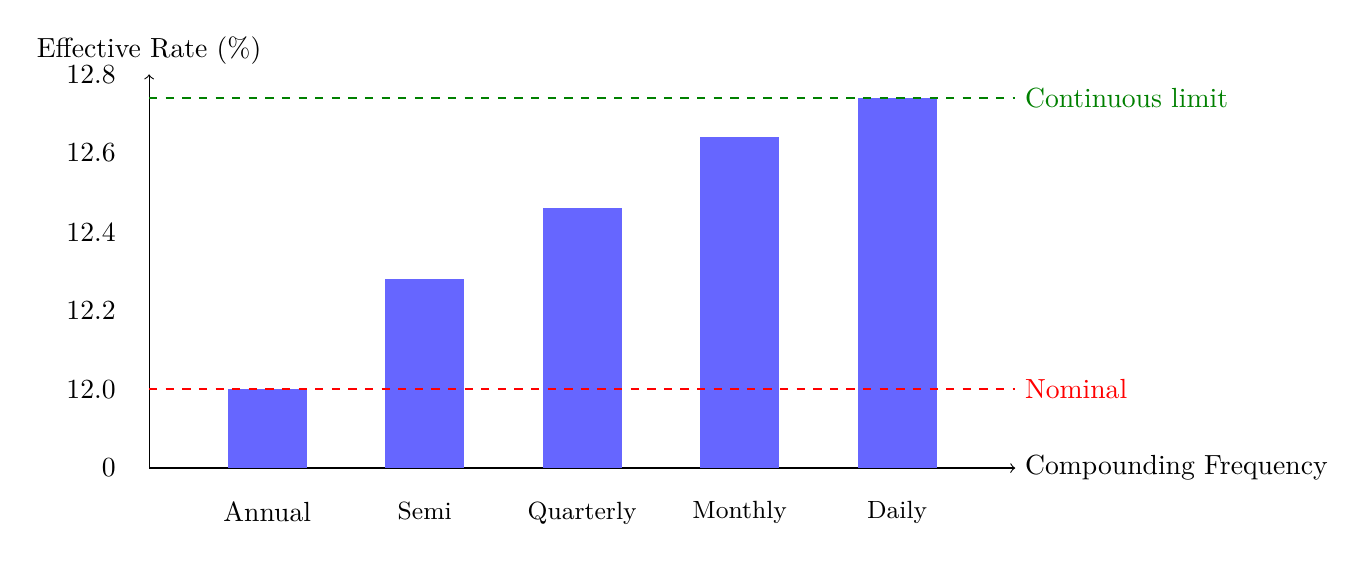
\begin{tikzpicture}[scale=1.0]
% Axes
\draw[->] (0,0) -- (11,0) node[right] {Compounding Frequency};
\draw[->] (0,0) -- (0,5) node[above] {Effective Rate (\%)};

% Y-axis labels
\foreach \y/\label in {0/0, 1/12.0, 2/12.2, 3/12.4, 4/12.6, 5/12.8}
    \node[left] at (-0.3,\y) {\label};

% Bars
\fill[blue!60] (1,0) rectangle (2,1);
\node[below] at (1.5,-0.3) {Annual};

\fill[blue!60] (3,0) rectangle (4,2.4);
\node[below,font=\small] at (3.5,-0.3) {Semi};

\fill[blue!60] (5,0) rectangle (6,3.3);
\node[below,font=\small] at (5.5,-0.3) {Quarterly};

\fill[blue!60] (7,0) rectangle (8,4.2);
\node[below,font=\small] at (7.5,-0.3) {Monthly};

\fill[blue!60] (9,0) rectangle (10,4.7);
\node[below,font=\small] at (9.5,-0.3) {Daily};

% Reference line at 12%
\draw[red,dashed,thick] (0,1) -- (11,1);
\node[right,red] at (11,1) {Nominal};

% Asymptote
\draw[green!50!black,dashed,thick] (0,4.7) -- (11,4.7);
\node[right,green!50!black] at (11,4.7) {Continuous limit};
\end{tikzpicture}
\end{figure}

\section{Continuous Compounding}\label{continuous-compounding}

As compounding becomes more frequent, the effective rate approaches a
limit:

\begin{tcolorbox}[enhanced jigsaw, toptitle=1mm, colbacktitle=quarto-callout-note-color!10!white, opacityback=0, leftrule=.75mm, breakable, colframe=quarto-callout-note-color-frame, toprule=.15mm, opacitybacktitle=0.6, coltitle=black, bottomrule=.15mm, colback=white, arc=.35mm, titlerule=0mm, rightrule=.15mm, left=2mm, title=\textcolor{quarto-callout-note-color}{\faInfo}\hspace{0.5em}{Definition: Continuous Compounding}, bottomtitle=1mm]

When interest compounds \textbf{continuously} (infinitely often), the
accumulation formula becomes:

\[
FV = PV \times e^{rt}
\]

Where: - \(e \approx 2.71828\) (Euler's number) - \(r\) = continuously
compounded rate - \(t\) = time

\end{tcolorbox}

\subsection{Example: Continuous
vs.~Annual}\label{example-continuous-vs.-annual}

\textbf{Invest \$1,000 at 10\% for 3 years:}

\begin{longtable}[]{@{}lll@{}}
\toprule\noalign{}
Compounding & Formula & Future Value \\
\midrule\noalign{}
\endhead
\bottomrule\noalign{}
\endlastfoot
Annual & \(1000 \times (1.10)^3\) & \textbf{\$1,331.00} \\
Continuous & \(1000 \times e^{0.10 \times 3}\) & \textbf{\$1,349.86} \\
\end{longtable}

\textbf{Difference}: \$1,349.86 − \$1,331.00 = \textbf{\$18.86} extra
from continuous compounding.

\section{Interest Rate Decomposition}\label{interest-rate-decomposition}

Real-world interest rates have multiple components:

\begin{tcolorbox}[enhanced jigsaw, toptitle=1mm, colbacktitle=quarto-callout-important-color!10!white, opacityback=0, leftrule=.75mm, breakable, colframe=quarto-callout-important-color-frame, toprule=.15mm, opacitybacktitle=0.6, coltitle=black, bottomrule=.15mm, colback=white, arc=.35mm, titlerule=0mm, rightrule=.15mm, left=2mm, title=\textcolor{quarto-callout-important-color}{\faExclamation}\hspace{0.5em}{Interest Rate Components}, bottomtitle=1mm]

\[
i = r_f + \text{inflation} + \text{risk premium} + \text{liquidity premium}
\]

Where: - \textbf{\(r_f\)}: Real risk-free rate (time preference) -
\textbf{Inflation}: Compensation for loss of purchasing power -
\textbf{Risk premium}: Compensation for default risk - \textbf{Liquidity
premium}: Compensation for illiquidity

\end{tcolorbox}

\subsection{Example: Corporate Bond
Rate}\label{example-corporate-bond-rate}

A corporate bond might have:

\begin{itemize}
\tightlist
\item
  Risk-free rate: 2\%
\item
  Expected inflation: 3\%
\item
  Default risk premium: 2\%
\item
  Liquidity premium: 1\%
\end{itemize}

\textbf{Total rate}: 2\% + 3\% + 2\% + 1\% = \textbf{8\%}

\section{Present Value of Annuities}\label{present-value-of-annuities}

A common cashflow pattern is an \textbf{annuity}: equal payments at
regular intervals.

\begin{tcolorbox}[enhanced jigsaw, toptitle=1mm, colbacktitle=quarto-callout-note-color!10!white, opacityback=0, leftrule=.75mm, breakable, colframe=quarto-callout-note-color-frame, toprule=.15mm, opacitybacktitle=0.6, coltitle=black, bottomrule=.15mm, colback=white, arc=.35mm, titlerule=0mm, rightrule=.15mm, left=2mm, title=\textcolor{quarto-callout-note-color}{\faInfo}\hspace{0.5em}{Definition: Annuity}, bottomtitle=1mm]

An \textbf{annuity} is a series of equal payments \(C\) made at regular
intervals for \(n\) periods.

\textbf{Present value of an annuity}:

\[
PV = C \times \frac{1 - v^n}{i} = C \times \frac{1 - (1+i)^{-n}}{i}
\]

This is often denoted as \(PV = C \times a_{\overline{n}|i}\) where
\(a_{\overline{n}|i}\) is the annuity factor.

\end{tcolorbox}

\subsection{Example: Mortgage Payment}\label{example-mortgage-payment}

\textbf{You take a \$200,000 mortgage at 5\% for 30 years. What's the
monthly payment?}

Given: - \(PV = 200,000\) - \(i = 5\% / 12 = 0.4167\%\) per month -
\(n = 30 \times 12 = 360\) months

Rearranging: \(C = PV \times \frac{i}{1 - (1+i)^{-n}}\)

\[
C = 200,000 \times \frac{0.004167}{1 - (1.004167)^{-360}} = 200,000 \times 0.00537 = \$1,073.64
\]

\textbf{Your monthly payment}: \textbf{\$1,073.64}

\subsection{Annuity Timeline}\label{annuity-timeline}

\begin{figure}[h]
\centering
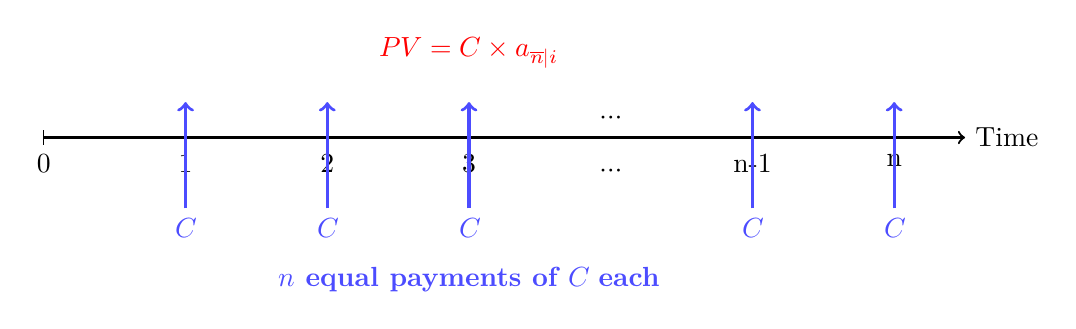
\begin{tikzpicture}[scale=0.9]
% Time axis
\draw[thick,->] (0,0) -- (13,0) node[right] {Time};
\foreach \x/\label in {0/0, 2/1, 4/2, 6/3, 10/n-1, 12/n}
    \draw (\x,0.1) -- (\x,-0.1) node[below] {\label};

% Equal payments
\foreach \x in {2,4,6,10,12} {
    \draw[->,blue!70,very thick] (\x,-1) -- (\x,0.5);
    \node[below,blue!70] at (\x,-1) {$C$};
}

% Dots
\node at (8,0.25) {$\cdots$};
\node at (8,-0.5) {$\cdots$};

% Label
\node[blue!70,font=\bfseries] at (6,-2) {$n$ equal payments of $C$ each};
\node[red,font=\bfseries] at (6,1.2) {$PV = C \times a_{\overline{n}|i}$};
\end{tikzpicture}
\end{figure}

\FloatBarrier

\section{Perpetuity: The Infinite
Annuity}\label{perpetuity-the-infinite-annuity}

\begin{tcolorbox}[enhanced jigsaw, toptitle=1mm, colbacktitle=quarto-callout-note-color!10!white, opacityback=0, leftrule=.75mm, breakable, colframe=quarto-callout-note-color-frame, toprule=.15mm, opacitybacktitle=0.6, coltitle=black, bottomrule=.15mm, colback=white, arc=.35mm, titlerule=0mm, rightrule=.15mm, left=2mm, title=\textcolor{quarto-callout-note-color}{\faInfo}\hspace{0.5em}{Definition: Perpetuity}, bottomtitle=1mm]

A \textbf{perpetuity} is an annuity that continues forever.

\textbf{Present value}:

\[
PV = \frac{C}{i}
\]

As \(n \to \infty\), the annuity formula simplifies to this beautifully
simple result.

\end{tcolorbox}

\subsection{Example: Preferred Stock}\label{example-preferred-stock}

A preferred stock pays \$5 per share annually forever. If the required
return is 8\%, what's it worth?

\[
PV = \frac{5}{0.08} = \$62.50
\]

\section{Summary Table: Key Formulas}\label{summary-table-key-formulas}

\begin{longtable}[]{@{}
  >{\raggedright\arraybackslash}p{(\linewidth - 4\tabcolsep) * \real{0.3913}}
  >{\raggedright\arraybackslash}p{(\linewidth - 4\tabcolsep) * \real{0.3913}}
  >{\raggedright\arraybackslash}p{(\linewidth - 4\tabcolsep) * \real{0.2174}}@{}}
\toprule\noalign{}
\begin{minipage}[b]{\linewidth}\raggedright
Concept
\end{minipage} & \begin{minipage}[b]{\linewidth}\raggedright
Formula
\end{minipage} & \begin{minipage}[b]{\linewidth}\raggedright
Use
\end{minipage} \\
\midrule\noalign{}
\endhead
\bottomrule\noalign{}
\endlastfoot
\textbf{Accumulation} & \(FV = PV \times (1+i)^t\) & Growing money
forward \\
\textbf{Discount} & \(PV = FV \times (1+i)^{-t}\) & Bringing money to
present \\
\textbf{Discount factor} & \(v = \frac{1}{1+i}\) & One-period
discounting \\
\textbf{Effective rate} & \((1 + i_m/m)^m - 1\) & Accounting for
compounding \\
\textbf{Continuous} & \(FV = PV \times e^{rt}\) & Continuous
compounding \\
\textbf{Annuity PV} & \(C \times \frac{1-v^n}{i}\) & Series of equal
payments \\
\textbf{Perpetuity PV} & \(\frac{C}{i}\) & Forever payments \\
\end{longtable}

\FloatBarrier

\section{Practical Insights}\label{practical-insights-1}

\begin{tcolorbox}[enhanced jigsaw, toptitle=1mm, colbacktitle=quarto-callout-important-color!10!white, opacityback=0, leftrule=.75mm, breakable, colframe=quarto-callout-important-color-frame, toprule=.15mm, opacitybacktitle=0.6, coltitle=black, bottomrule=.15mm, colback=white, arc=.35mm, titlerule=0mm, rightrule=.15mm, left=2mm, title=\textcolor{quarto-callout-important-color}{\faExclamation}\hspace{0.5em}{Using the Right Rate}, bottomtitle=1mm]

\textbf{Always match}: - \textbf{Time period} of cashflows (monthly,
annual, etc.) - \textbf{Compounding frequency} of the rate -
\textbf{Risk level} (risk-free rate vs.~risky rate)

Example: For monthly mortgage payments, use monthly interest rate, not
annual.

\end{tcolorbox}

\begin{tcolorbox}[enhanced jigsaw, toptitle=1mm, colbacktitle=quarto-callout-warning-color!10!white, opacityback=0, leftrule=.75mm, breakable, colframe=quarto-callout-warning-color-frame, toprule=.15mm, opacitybacktitle=0.6, coltitle=black, bottomrule=.15mm, colback=white, arc=.35mm, titlerule=0mm, rightrule=.15mm, left=2mm, title=\textcolor{quarto-callout-warning-color}{\faExclamationTriangle}\hspace{0.5em}{Common Mistakes}, bottomtitle=1mm]

\begin{enumerate}
\def\labelenumi{\arabic{enumi}.}
\tightlist
\item
  \textbf{Mixing rates}: Using annual rate for monthly cashflows
\item
  \textbf{Forgetting compounding}: Treating 6\% semi-annual as 6\%
  annual
\item
  \textbf{Wrong perspective}: Confusing investor vs.~borrower viewpoint
\item
  \textbf{Sign errors}: Getting cashflow directions backward
\end{enumerate}

\end{tcolorbox}

\section{Summary}\label{summary-3}

✅ \textbf{Interest rate} \(i\) = price of time, quantifies time value
of money\\
✅ \textbf{Accumulation} (forward) vs.~\textbf{Discount} (backward) =
two directions\\
✅ \textbf{Compound interest} = interest on interest (grows
exponentially)\\
✅ \textbf{Effective rate} accounts for compounding frequency\\
✅ \textbf{Continuous compounding} = infinite frequency limit\\
✅ \textbf{Annuities} = equal periodic payments (closed-form PV
formula)\\
✅ \textbf{Perpetuities} = infinite annuities (\(PV = C/i\))

\begin{tcolorbox}[enhanced jigsaw, toptitle=1mm, colbacktitle=quarto-callout-caution-color!10!white, opacityback=0, leftrule=.75mm, breakable, colframe=quarto-callout-caution-color-frame, toprule=.15mm, opacitybacktitle=0.6, coltitle=black, bottomrule=.15mm, colback=white, arc=.35mm, titlerule=0mm, rightrule=.15mm, left=2mm, title=\textcolor{quarto-callout-caution-color}{\faFire}\hspace{0.5em}{References}, bottomtitle=1mm]

\textbf{Book:} Pearson Corporate Finance 6th Edition, Chapter 5
(Interest Rates), Page 149,
\href{https://cdn.jsdelivr.net/gh/mrbungie/financial_maths@main/resources/books/pearson_corporate_finance_6th.pdf\#page=149}{Direct
Link}

\textbf{Slide:} Financial Mathematics Slides 1-96, Slides 37-93 (Module
2: Financial Laws - Interest, discount, accumulation factors, simple \&
compound interest), Page 37,
\href{https://cdn.jsdelivr.net/gh/mrbungie/financial_maths@main/resources/slideshows/25_09_30_FinancialMathematics_Slides_1_96.pdf\#page=37}{Direct
Link}

\end{tcolorbox}

\begin{center}\rule{0.5\linewidth}{0.5pt}\end{center}

\textbf{Next}: Check out the \href{cheat_sheet.qmd}{Cheat Sheet} for a
one-page reference of all key formulas!

\bookmarksetup{startatroot}

\chapter*{Cheat Sheet}\label{cheat-sheet}
\addcontentsline{toc}{chapter}{Cheat Sheet}

\markboth{Cheat Sheet}{Cheat Sheet}

\begin{tcolorbox}[enhanced jigsaw, toptitle=1mm, colbacktitle=quarto-callout-note-color!10!white, opacityback=0, leftrule=.75mm, breakable, colframe=quarto-callout-note-color-frame, toprule=.15mm, opacitybacktitle=0.6, coltitle=black, bottomrule=.15mm, colback=white, arc=.35mm, titlerule=0mm, rightrule=.15mm, left=2mm, title={📋 Quick Reference Guide}, bottomtitle=1mm]

This one-page summary contains all essential formulas, conventions, and
concepts from Financial Mathematics Class 1.

\end{tcolorbox}

\begin{center}\rule{0.5\linewidth}{0.5pt}\end{center}

\section*{🔢 Core Formulas}\label{core-formulas}
\addcontentsline{toc}{section}{🔢 Core Formulas}

\markright{🔢 Core Formulas}

\subsection*{Time Value of Money}\label{time-value-of-money}
\addcontentsline{toc}{subsection}{Time Value of Money}

\begin{longtable}[]{@{}
  >{\raggedright\arraybackslash}p{(\linewidth - 4\tabcolsep) * \real{0.3103}}
  >{\raggedright\arraybackslash}p{(\linewidth - 4\tabcolsep) * \real{0.3103}}
  >{\raggedright\arraybackslash}p{(\linewidth - 4\tabcolsep) * \real{0.3793}}@{}}
\toprule\noalign{}
\begin{minipage}[b]{\linewidth}\raggedright
Concept
\end{minipage} & \begin{minipage}[b]{\linewidth}\raggedright
Formula
\end{minipage} & \begin{minipage}[b]{\linewidth}\raggedright
Variables
\end{minipage} \\
\midrule\noalign{}
\endhead
\bottomrule\noalign{}
\endlastfoot
\textbf{Future Value} & \(FV = PV \times (1+i)^t\) & \(PV\) = present
value\(i\) = interest rate\(t\) = time \\
\textbf{Present Value} & \(PV = \frac{FV}{(1+i)^t}\) & \(FV\) = future
value \\
\textbf{Discount Factor} & \(v = \frac{1}{1+i}\) or
\(v^t = \frac{1}{(1+i)^t}\) & \(v\) = one-period discount \\
\textbf{Accumulation Factor} & \(a(t) = (1+i)^t\) & Growth multiplier \\
\end{longtable}

\subsection*{Net Present Value}\label{net-present-value}
\addcontentsline{toc}{subsection}{Net Present Value}

\[
\text{NPV} = \sum_{t=0}^{n} \frac{C_t}{(1+i)^t}
\]

\textbf{Decision Rule}: Accept if NPV \textgreater{} 0, Reject if NPV
\textless{} 0

\subsection*{Value Function}\label{value-function-1}
\addcontentsline{toc}{subsection}{Value Function}

\[
V(t) = \sum_{t_i \leq t} C_i \cdot (1+i)^{t-t_i} + \sum_{t_j > t} \frac{C_j}{(1+i)^{t_j - t}}
\]

\begin{itemize}
\tightlist
\item
  First sum: Past cashflows accumulated to \(t\)
\item
  Second sum: Future cashflows discounted to \(t\)
\end{itemize}

\begin{center}\rule{0.5\linewidth}{0.5pt}\end{center}

\section*{💰 Annuities \& Perpetuities}\label{annuities-perpetuities}
\addcontentsline{toc}{section}{💰 Annuities \& Perpetuities}

\markright{💰 Annuities \& Perpetuities}

\begin{longtable}[]{@{}
  >{\raggedright\arraybackslash}p{(\linewidth - 4\tabcolsep) * \real{0.2143}}
  >{\raggedright\arraybackslash}p{(\linewidth - 4\tabcolsep) * \real{0.3214}}
  >{\raggedright\arraybackslash}p{(\linewidth - 4\tabcolsep) * \real{0.4643}}@{}}
\toprule\noalign{}
\begin{minipage}[b]{\linewidth}\raggedright
Type
\end{minipage} & \begin{minipage}[b]{\linewidth}\raggedright
Formula
\end{minipage} & \begin{minipage}[b]{\linewidth}\raggedright
Description
\end{minipage} \\
\midrule\noalign{}
\endhead
\bottomrule\noalign{}
\endlastfoot
\textbf{Annuity PV} & \(PV = C \times \frac{1 - v^n}{i}\) & \(n\) equal
payments of \(C\) \\
\textbf{Annuity Factor} & \(a_{\overline{n}|i} = \frac{1 - v^n}{i}\) &
Standard notation \\
\textbf{Perpetuity PV} & \(PV = \frac{C}{i}\) & Infinite equal
payments \\
\textbf{Growing Perpetuity} & \(PV = \frac{C}{i - g}\) & Growth rate
\(g < i\) \\
\end{longtable}

\FloatBarrier

\begin{center}\rule{0.5\linewidth}{0.5pt}\end{center}

\section*{📊 Interest Rate Conventions}\label{interest-rate-conventions}
\addcontentsline{toc}{section}{📊 Interest Rate Conventions}

\markright{📊 Interest Rate Conventions}

\subsection*{Effective Annual Rate}\label{effective-annual-rate}
\addcontentsline{toc}{subsection}{Effective Annual Rate}

\[
\text{EAR} = \left(1 + \frac{r}{m}\right)^m - 1
\]

Where: \(r\) = nominal rate, \(m\) = compounding periods per year

\subsection*{Compounding Frequencies}\label{compounding-frequencies}
\addcontentsline{toc}{subsection}{Compounding Frequencies}

\begin{longtable}[]{@{}lll@{}}
\toprule\noalign{}
Frequency & \(m\) & Example (12\% nominal) \\
\midrule\noalign{}
\endhead
\bottomrule\noalign{}
\endlastfoot
Annual & 1 & 12.00\% effective \\
Semi-annual & 2 & 12.36\% effective \\
Quarterly & 4 & 12.55\% effective \\
Monthly & 12 & 12.68\% effective \\
Continuous & ∞ & \(e^{0.12} - 1 = 12.75\%\) \\
\end{longtable}

\FloatBarrier

\subsection*{Continuous Compounding}\label{continuous-compounding-1}
\addcontentsline{toc}{subsection}{Continuous Compounding}

\[
FV = PV \times e^{rt} \quad \text{and} \quad PV = FV \times e^{-rt}
\]

\begin{center}\rule{0.5\linewidth}{0.5pt}\end{center}

\section*{📅 Day Count Conventions}\label{day-count-conventions-1}
\addcontentsline{toc}{section}{📅 Day Count Conventions}

\markright{📅 Day Count Conventions}

\begin{longtable}[]{@{}llll@{}}
\toprule\noalign{}
Convention & Year & Period Calculation & Usage \\
\midrule\noalign{}
\endhead
\bottomrule\noalign{}
\endlastfoot
\textbf{ACT/ACT} & Actual days (365/366) & Actual days & US
Treasuries \\
\textbf{ACT/360} & 360 days & Actual days & Money markets, loans \\
\textbf{30/360} & 360 days & 30 days/month & Corporate bonds \\
\end{longtable}

\FloatBarrier

\subsection*{Accrued Interest}\label{accrued-interest}
\addcontentsline{toc}{subsection}{Accrued Interest}

\[
\text{AI} = C \times \frac{\text{days since last coupon}}{\text{days in period}}
\]

\begin{center}\rule{0.5\linewidth}{0.5pt}\end{center}

\section*{🎯 Bond Pricing}\label{bond-pricing}
\addcontentsline{toc}{section}{🎯 Bond Pricing}

\markright{🎯 Bond Pricing}

\subsection*{Components}\label{components}
\addcontentsline{toc}{subsection}{Components}

\begin{longtable}[]{@{}
  >{\raggedright\arraybackslash}p{(\linewidth - 2\tabcolsep) * \real{0.3333}}
  >{\raggedright\arraybackslash}p{(\linewidth - 2\tabcolsep) * \real{0.6667}}@{}}
\toprule\noalign{}
\begin{minipage}[b]{\linewidth}\raggedright
Term
\end{minipage} & \begin{minipage}[b]{\linewidth}\raggedright
Definition
\end{minipage} \\
\midrule\noalign{}
\endhead
\bottomrule\noalign{}
\endlastfoot
\textbf{Face Value} & Principal repaid at maturity (typically
\$1,000) \\
\textbf{Coupon Rate} & Annual interest rate on face value \\
\textbf{Coupon Payment} &
\(C = \text{Face Value} \times \text{Coupon Rate}\) \\
\textbf{Clean Price} & Quoted price (excludes accrued interest) \\
\textbf{Dirty Price} & Invoice price = Clean + Accrued Interest \\
\end{longtable}

\subsection*{Bond Cashflow Pattern}\label{bond-cashflow-pattern}
\addcontentsline{toc}{subsection}{Bond Cashflow Pattern}

\textbf{Timeline}: Initial payment (buy bond) → periodic coupons → final
coupon + face value repayment

\begin{center}\rule{0.5\linewidth}{0.5pt}\end{center}

\section*{💵 Cashflow Conventions}\label{cashflow-conventions}
\addcontentsline{toc}{section}{💵 Cashflow Conventions}

\markright{💵 Cashflow Conventions}

\subsection*{Sign Convention}\label{sign-convention}
\addcontentsline{toc}{subsection}{Sign Convention}

\begin{longtable}[]{@{}
  >{\raggedright\arraybackslash}p{(\linewidth - 4\tabcolsep) * \real{0.3667}}
  >{\raggedright\arraybackslash}p{(\linewidth - 4\tabcolsep) * \real{0.2000}}
  >{\raggedright\arraybackslash}p{(\linewidth - 4\tabcolsep) * \real{0.4333}}@{}}
\toprule\noalign{}
\begin{minipage}[b]{\linewidth}\raggedright
Direction
\end{minipage} & \begin{minipage}[b]{\linewidth}\raggedright
Sign
\end{minipage} & \begin{minipage}[b]{\linewidth}\raggedright
Perspective
\end{minipage} \\
\midrule\noalign{}
\endhead
\bottomrule\noalign{}
\endlastfoot
\textbf{Inflow} (receive) & \textbf{+} (positive) & {● Green ↑} \\
\textbf{Outflow} (pay) & \textbf{−} (negative) & {● Red ↓} \\
\end{longtable}

\begin{tcolorbox}[enhanced jigsaw, toptitle=1mm, colbacktitle=quarto-callout-warning-color!10!white, opacityback=0, leftrule=.75mm, breakable, colframe=quarto-callout-warning-color-frame, toprule=.15mm, opacitybacktitle=0.6, coltitle=black, bottomrule=.15mm, colback=white, arc=.35mm, titlerule=0mm, rightrule=.15mm, left=2mm, title=\textcolor{quarto-callout-warning-color}{\faExclamationTriangle}\hspace{0.5em}{Warning}, bottomtitle=1mm]

\textbf{Critical}: Always establish whose perspective (investor,
borrower, company, etc.) and maintain consistency!

\end{tcolorbox}

\subsection*{Cashflow Patterns}\label{cashflow-patterns}
\addcontentsline{toc}{subsection}{Cashflow Patterns}

\begin{longtable}[]{@{}lll@{}}
\toprule\noalign{}
Pattern & Structure & Example \\
\midrule\noalign{}
\endhead
\bottomrule\noalign{}
\endlastfoot
\textbf{Investment} & − then + & Buy stock, then dividends + sale \\
\textbf{Financing} & + then − & Receive loan, then repayments \\
\end{longtable}

\begin{center}\rule{0.5\linewidth}{0.5pt}\end{center}

\section*{🔄 Relationship Diagram}\label{relationship-diagram}
\addcontentsline{toc}{section}{🔄 Relationship Diagram}

\markright{🔄 Relationship Diagram}

\begin{figure}[h]
\centering
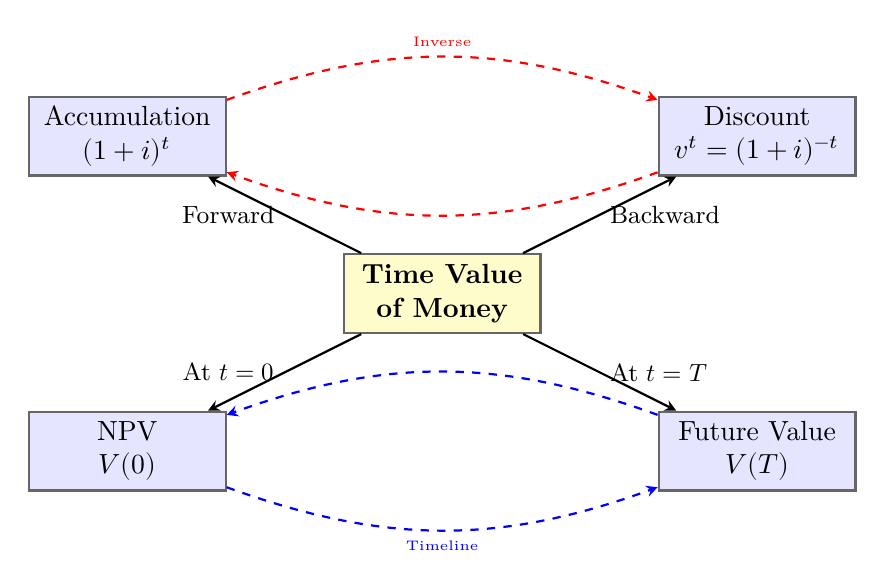
\begin{tikzpicture}[
    box/.style={rectangle, draw=black!60, fill=blue!10, thick, minimum width=2.5cm, minimum height=1cm, align=center},
    arrow/.style={->, >=stealth, thick}
]

% Central concept
\node[box, fill=yellow!20] (tvm) at (5,2) {\textbf{Time Value}\\\textbf{of Money}};

% Surrounding concepts
\node[box] (acc) at (1,4) {Accumulation\\$(1+i)^t$};
\node[box] (disc) at (9,4) {Discount\\$v^t = (1+i)^{-t}$};
\node[box] (npv) at (1,0) {NPV\\$V(0)$};
\node[box] (fv) at (9,0) {Future Value\\$V(T)$};

% Arrows
\draw[arrow] (tvm) -- (acc) node[midway,left,font=\small] {Forward};
\draw[arrow] (tvm) -- (disc) node[midway,right,font=\small] {Backward};
\draw[arrow] (tvm) -- (npv) node[midway,left,font=\small] {At $t=0$};
\draw[arrow] (tvm) -- (fv) node[midway,right,font=\small] {At $t=T$};

% Connecting arrows
\draw[arrow, dashed, red] (acc) to[bend left=20] node[above,font=\tiny] {Inverse} (disc);
\draw[arrow, dashed, red] (disc) to[bend left=20] (acc);
\draw[arrow, dashed, blue] (npv) to[bend right=20] node[below,font=\tiny] {Timeline} (fv);
\draw[arrow, dashed, blue] (fv) to[bend right=20] (npv);
\end{tikzpicture}
\end{figure}

\FloatBarrier

\begin{center}\rule{0.5\linewidth}{0.5pt}\end{center}

\section*{🧮 Quick Calculations}\label{quick-calculations}
\addcontentsline{toc}{section}{🧮 Quick Calculations}

\markright{🧮 Quick Calculations}

\subsection*{Rule of 72 (Approximation)}\label{rule-of-72-approximation}
\addcontentsline{toc}{subsection}{Rule of 72 (Approximation)}

\textbf{Time to double} \(\approx \frac{72}{\text{interest rate (\%)}}\)

Example: At 6\% interest, money doubles in \(\approx 72/6 = 12\) years.

\subsection*{Exact Doubling Time}\label{exact-doubling-time}
\addcontentsline{toc}{subsection}{Exact Doubling Time}

\[
t = \frac{\ln(2)}{\ln(1+i)}
\]

\begin{center}\rule{0.5\linewidth}{0.5pt}\end{center}

\section*{🎨 Timeline Icons}\label{timeline-icons}
\addcontentsline{toc}{section}{🎨 Timeline Icons}

\markright{🎨 Timeline Icons}

Quick reference for drawing cashflow diagrams:

\begin{longtable}[]{@{}ll@{}}
\toprule\noalign{}
Symbol & Meaning \\
\midrule\noalign{}
\endhead
\bottomrule\noalign{}
\endlastfoot
→ & Time axis (left to right) \\
{↑} & Inflow (positive cashflow) \\
{↓} & Outflow (negative cashflow) \\
● & Point in time \\
\textbar--\textbar{} & Time period/interval \\
\end{longtable}

\begin{center}\rule{0.5\linewidth}{0.5pt}\end{center}

\section*{⚠️ Common Pitfalls}\label{common-pitfalls}
\addcontentsline{toc}{section}{⚠️ Common Pitfalls}

\markright{⚠️ Common Pitfalls}

\begin{tcolorbox}[enhanced jigsaw, toptitle=1mm, colbacktitle=quarto-callout-warning-color!10!white, opacityback=0, leftrule=.75mm, breakable, colframe=quarto-callout-warning-color-frame, toprule=.15mm, opacitybacktitle=0.6, coltitle=black, bottomrule=.15mm, colback=white, arc=.35mm, titlerule=0mm, rightrule=.15mm, left=2mm, title=\textcolor{quarto-callout-warning-color}{\faExclamationTriangle}\hspace{0.5em}{Mistakes to Avoid}, bottomtitle=1mm]

\begin{enumerate}
\def\labelenumi{\arabic{enumi}.}
\tightlist
\item
  \textbf{Sign errors}: Mixing up inflows and outflows
\item
  \textbf{Period mismatch}: Using annual rate with monthly cashflows
\item
  \textbf{Perspective confusion}: Switching between investor/borrower
  view mid-calculation
\item
  \textbf{Forgetting compounding}: Treating \(6\%\) semi-annual as
  \(6\%\) annual
\item
  \textbf{Wrong discount rate}: Using risk-free rate for risky cashflows
\item
  \textbf{NPV timing}: Forgetting that NPV is at \(t=0\), not \(t=1\)
\end{enumerate}

\end{tcolorbox}

\begin{center}\rule{0.5\linewidth}{0.5pt}\end{center}

\section*{📈 Key Relationships}\label{key-relationships}
\addcontentsline{toc}{section}{📈 Key Relationships}

\markright{📈 Key Relationships}

\subsection*{Interest Rate Components}\label{interest-rate-components-1}
\addcontentsline{toc}{subsection}{Interest Rate Components}

\[
i_{\text{total}} = r_{\text{real}} + \pi_{\text{expected}} + \text{risk premium} + \text{liquidity premium}
\]

\subsection*{Fisher Equation}\label{fisher-equation}
\addcontentsline{toc}{subsection}{Fisher Equation}

\[
1 + i_{\text{nominal}} = (1 + r_{\text{real}})(1 + \pi)
\]

Approximation: \(i \approx r + \pi\)

\begin{center}\rule{0.5\linewidth}{0.5pt}\end{center}

\section*{🎓 Exam Tips}\label{exam-tips}
\addcontentsline{toc}{section}{🎓 Exam Tips}

\markright{🎓 Exam Tips}

\subsection*{Quick Checks}\label{quick-checks}
\addcontentsline{toc}{subsection}{Quick Checks}

\begin{enumerate}
\def\labelenumi{\arabic{enumi}.}
\tightlist
\item
  \textbf{Units}: All rates and times in consistent units (annual with
  annual, monthly with monthly)
\item
  \textbf{Signs}: Do a sanity check---are you paying or receiving?
\item
  \textbf{Magnitudes}: Does your answer make sense? (e.g., NPV shouldn't
  be 1000× the cashflows)
\item
  \textbf{Zero test}: If \(i=0\), formulas should reduce to simple sums
\end{enumerate}

\subsection*{Calculator Shortcuts}\label{calculator-shortcuts}
\addcontentsline{toc}{subsection}{Calculator Shortcuts}

\begin{itemize}
\tightlist
\item
  \textbf{Compound interest}: Use \((1+i)^t\) directly, not repeated
  multiplication
\item
  \textbf{NPV}: Most financial calculators have built-in NPV function
\item
  \textbf{Annuities}: Use annuity factor formula, not term-by-term
\end{itemize}

\begin{center}\rule{0.5\linewidth}{0.5pt}\end{center}

\section*{📚 Formula Summary Card}\label{formula-summary-card}
\addcontentsline{toc}{section}{📚 Formula Summary Card}

\markright{📚 Formula Summary Card}

\begin{tcolorbox}[enhanced jigsaw, toptitle=1mm, colbacktitle=quarto-callout-note-color!10!white, opacityback=0, leftrule=.75mm, breakable, colframe=quarto-callout-note-color-frame, toprule=.15mm, opacitybacktitle=0.6, coltitle=black, bottomrule=.15mm, colback=white, arc=.35mm, titlerule=0mm, rightrule=.15mm, left=2mm, title={The ``Big 7'' Formulas}, bottomtitle=1mm]

\begin{enumerate}
\def\labelenumi{\arabic{enumi}.}
\tightlist
\item
  \(FV = PV \times (1+i)^t\) --- Future value
\item
  \(PV = \frac{FV}{(1+i)^t}\) --- Present value\\
\item
  \(\text{NPV} = \sum \frac{C_t}{(1+i)^t}\) --- Net present value\\
\item
  \(\text{EAR} = (1 + r/m)^m - 1\) --- Effective rate\\
\item
  \(PV_{\text{annuity}} = C \times \frac{1-v^n}{i}\) --- Annuity\\
\item
  \(PV_{\text{perpetuity}} = \frac{C}{i}\) --- Perpetuity\\
\item
  \(\text{Dirty Price} = \text{Clean Price} + \text{Accrued Interest}\)
  --- Bonds
\end{enumerate}

\textbf{Master these, and you've mastered the course!}

\end{tcolorbox}

\begin{center}\rule{0.5\linewidth}{0.5pt}\end{center}

\begin{tcolorbox}[enhanced jigsaw, toptitle=1mm, colbacktitle=quarto-callout-tip-color!10!white, opacityback=0, leftrule=.75mm, breakable, colframe=quarto-callout-tip-color-frame, toprule=.15mm, opacitybacktitle=0.6, coltitle=black, bottomrule=.15mm, colback=white, arc=.35mm, titlerule=0mm, rightrule=.15mm, left=2mm, title=\textcolor{quarto-callout-tip-color}{\faLightbulb}\hspace{0.5em}{💡 Pro Tip}, bottomtitle=1mm]

Print this page and keep it handy during problem-solving. Better yet,
recreate it by hand to reinforce your understanding!

\end{tcolorbox}

\begin{tcolorbox}[enhanced jigsaw, toptitle=1mm, colbacktitle=quarto-callout-caution-color!10!white, opacityback=0, leftrule=.75mm, breakable, colframe=quarto-callout-caution-color-frame, toprule=.15mm, opacitybacktitle=0.6, coltitle=black, bottomrule=.15mm, colback=white, arc=.35mm, titlerule=0mm, rightrule=.15mm, left=2mm, title=\textcolor{quarto-callout-caution-color}{\faFire}\hspace{0.5em}{References}, bottomtitle=1mm]

This cheat sheet consolidates material from all chapters:

\textbf{Book:} Pearson Corporate Finance 6th Edition, Chapters 3-6 (Part
2: Time, Money, and Interest Rates), Page 103,
\href{https://cdn.jsdelivr.net/gh/mrbungie/financial_maths@main/resources/books/pearson_corporate_finance_6th.pdf\#page=103}{Direct
Link}

\textbf{Slide:} Financial Mathematics Slides 1-96, Complete Modules 1-2
(Basic Notions \& Financial Laws), Page 1,
\href{https://cdn.jsdelivr.net/gh/mrbungie/financial_maths@main/resources/slideshows/25_09_30_FinancialMathematics_Slides_1_96.pdf\#page=1}{Direct
Link}

\end{tcolorbox}

\begin{center}\rule{0.5\linewidth}{0.5pt}\end{center}

\textbf{Ready to Practice?} Head to \href{exercises.qmd}{Exercises} to
test your knowledge!

\bookmarksetup{startatroot}

\chapter{Exercises}\label{exercises}

\section{Introduction}\label{introduction-4}

Practice is essential for mastering financial mathematics. These
exercises cover all major topics from the course. Work through them
carefully, and check your answers against the detailed solutions
provided.

\begin{tcolorbox}[enhanced jigsaw, toptitle=1mm, colbacktitle=quarto-callout-tip-color!10!white, opacityback=0, leftrule=.75mm, breakable, colframe=quarto-callout-tip-color-frame, toprule=.15mm, opacitybacktitle=0.6, coltitle=black, bottomrule=.15mm, colback=white, arc=.35mm, titlerule=0mm, rightrule=.15mm, left=2mm, title=\textcolor{quarto-callout-tip-color}{\faLightbulb}\hspace{0.5em}{How to Use These Exercises}, bottomtitle=1mm]

\begin{enumerate}
\def\labelenumi{\arabic{enumi}.}
\tightlist
\item
  \textbf{Try first without looking at solutions}
\item
  Show all your work (write out formulas, calculations)
\item
  Check units and signs carefully
\item
  Compare your approach with the solution method
\item
  If you get stuck, review the relevant chapter before checking the
  solution
\end{enumerate}

\end{tcolorbox}

\begin{center}\rule{0.5\linewidth}{0.5pt}\end{center}

\section{Exercise 1: Cashflow Table → Interest
Split}\label{exercise-1-cashflow-table-interest-split}

\begin{tcolorbox}[enhanced jigsaw, toptitle=1mm, colbacktitle=quarto-callout-note-color!10!white, opacityback=0, leftrule=.75mm, breakable, colframe=quarto-callout-note-color-frame, toprule=.15mm, opacitybacktitle=0.6, coltitle=black, bottomrule=.15mm, colback=white, arc=.35mm, titlerule=0mm, rightrule=.15mm, left=2mm, title=\textcolor{quarto-callout-note-color}{\faInfo}\hspace{0.5em}{Problem}, bottomtitle=1mm]

You've taken out a \textbf{3-year loan of \$10,000} at a \textbf{7\%
annual interest rate} with \textbf{fixed annual payments of \$3,810.52}.

Complete the amortization table below by filling in the missing values:

\begin{longtable}[]{@{}
  >{\raggedright\arraybackslash}p{(\linewidth - 8\tabcolsep) * \real{0.0896}}
  >{\raggedright\arraybackslash}p{(\linewidth - 8\tabcolsep) * \real{0.1343}}
  >{\raggedright\arraybackslash}p{(\linewidth - 8\tabcolsep) * \real{0.1493}}
  >{\raggedright\arraybackslash}p{(\linewidth - 8\tabcolsep) * \real{0.3134}}
  >{\raggedright\arraybackslash}p{(\linewidth - 8\tabcolsep) * \real{0.3134}}@{}}
\toprule\noalign{}
\begin{minipage}[b]{\linewidth}\raggedright
Year
\end{minipage} & \begin{minipage}[b]{\linewidth}\raggedright
Payment
\end{minipage} & \begin{minipage}[b]{\linewidth}\raggedright
Interest
\end{minipage} & \begin{minipage}[b]{\linewidth}\raggedright
Principal Repayment
\end{minipage} & \begin{minipage}[b]{\linewidth}\raggedright
Outstanding Balance
\end{minipage} \\
\midrule\noalign{}
\endhead
\bottomrule\noalign{}
\endlastfoot
0 & --- & --- & --- & 10,000.00 \\
1 & 3,810.52 & \textbf{?} & \textbf{?} & \textbf{?} \\
2 & 3,810.52 & \textbf{?} & \textbf{?} & \textbf{?} \\
3 & 3,810.52 & \textbf{?} & \textbf{?} & 0.00 \\
\end{longtable}

\FloatBarrier

\textbf{Related Chapter}: \hyperref[basic-notions]{Basic Notions}

\end{tcolorbox}

\subsection*{Solution}\label{solution}
\addcontentsline{toc}{subsection}{Solution}

\begin{tcolorbox}[enhanced jigsaw, toptitle=1mm, colbacktitle=quarto-callout-tip-color!10!white, opacityback=0, leftrule=.75mm, breakable, colframe=quarto-callout-tip-color-frame, toprule=.15mm, opacitybacktitle=0.6, coltitle=black, bottomrule=.15mm, colback=white, arc=.35mm, titlerule=0mm, rightrule=.15mm, left=2mm, title={Click to reveal solution}, bottomtitle=1mm]

\textbf{Key formulas}: - Interest for period = Outstanding balance at
start × interest rate - Principal repayment = Payment − Interest - New
balance = Old balance − Principal repayment

\textbf{Year 1}: - Interest: \(10,000 \times 0.07 = \$700.00\) -
Principal: \(3,810.52 - 700.00 = \$3,110.52\) - Balance:
\(10,000 - 3,110.52 = \$6,889.48\)

\textbf{Year 2}: - Interest: \(6,889.48 \times 0.07 = \$482.26\) -
Principal: \(3,810.52 - 482.26 = \$3,328.26\) - Balance:
\(6,889.48 - 3,328.26 = \$3,561.22\)

\textbf{Year 3}: - Interest: \(3,561.22 \times 0.07 = \$249.29\) -
Principal: \(3,810.52 - 249.29 = \$3,561.23\) (slight rounding) -
Balance: \(3,561.22 - 3,561.22 = \$0.00\)

\textbf{Completed Table}:

\begin{longtable}[]{@{}lllll@{}}
\toprule\noalign{}
Year & Payment & Interest & Principal & Outstanding Balance \\
\midrule\noalign{}
\endhead
\bottomrule\noalign{}
\endlastfoot
0 & --- & --- & --- & 10,000.00 \\
1 & 3,810.52 & 700.00 & 3,110.52 & 6,889.48 \\
2 & 3,810.52 & 482.26 & 3,328.26 & 3,561.22 \\
3 & 3,810.52 & 249.29 & 3,561.23 & 0.00 \\
\end{longtable}

\FloatBarrier

\textbf{Key insight}: Notice how interest decreases each year while
principal repayment increases---this is typical for fixed-payment loans.

\end{tcolorbox}

\begin{center}\rule{0.5\linewidth}{0.5pt}\end{center}

\section{Exercise 2: Bond Dirty
Price}\label{exercise-2-bond-dirty-price}

\begin{tcolorbox}[enhanced jigsaw, toptitle=1mm, colbacktitle=quarto-callout-note-color!10!white, opacityback=0, leftrule=.75mm, breakable, colframe=quarto-callout-note-color-frame, toprule=.15mm, opacitybacktitle=0.6, coltitle=black, bottomrule=.15mm, colback=white, arc=.35mm, titlerule=0mm, rightrule=.15mm, left=2mm, title=\textcolor{quarto-callout-note-color}{\faInfo}\hspace{0.5em}{Problem}, bottomtitle=1mm]

You're buying a \textbf{US Treasury bond} with the following
characteristics:

\begin{itemize}
\tightlist
\item
  \textbf{Face value}: \$1,000
\item
  \textbf{Coupon rate}: 5\% annual (paid semi-annually, so \$25 every 6
  months)
\item
  \textbf{Clean price}: Quoted at \textbf{98.75} (as \% of face value)
\item
  \textbf{Last coupon date}: January 15, 2025
\item
  \textbf{Settlement date} (purchase date): April 10, 2025
\item
  \textbf{Next coupon date}: July 15, 2025
\item
  \textbf{Day count convention}: ACT/ACT
\end{itemize}

\textbf{Questions}: 1. Calculate the \textbf{accrued interest} 2.
Calculate the \textbf{dirty price} (what you actually pay) 3. Draw a
timeline showing the accrued period

\textbf{Related Chapter}: \hyperref[bonds]{Bonds}

\end{tcolorbox}

\subsection*{Solution}\label{solution-1}
\addcontentsline{toc}{subsection}{Solution}

\begin{tcolorbox}[enhanced jigsaw, toptitle=1mm, colbacktitle=quarto-callout-tip-color!10!white, opacityback=0, leftrule=.75mm, breakable, colframe=quarto-callout-tip-color-frame, toprule=.15mm, opacitybacktitle=0.6, coltitle=black, bottomrule=.15mm, colback=white, arc=.35mm, titlerule=0mm, rightrule=.15mm, left=2mm, title={Click to reveal solution}, bottomtitle=1mm]

\textbf{Step 1: Count the days}

\begin{itemize}
\tightlist
\item
  Days from Jan 15 to Apr 10:

  \begin{itemize}
  \tightlist
  \item
    Jan 15 → Jan 31: 16 days
  \item
    February: 28 days (2025 is not a leap year)
  \item
    March: 31 days
  \item
    Apr 1 → Apr 10: 10 days
  \item
    \textbf{Total elapsed}: \(16 + 28 + 31 + 10 = 85\) days
  \end{itemize}
\item
  Days in full coupon period (Jan 15 → Jul 15):

  \begin{itemize}
  \tightlist
  \item
    Using same method: 181 days
  \end{itemize}
\end{itemize}

\textbf{Step 2: Calculate accrued interest}

\[
\text{Accrued Interest} = \$25 \times \frac{85}{181} = \$25 \times 0.4696 = \$11.74
\]

\textbf{Step 3: Calculate clean price in dollars}

\[
\text{Clean Price} = 98.75\% \times \$1,000 = \$987.50
\]

\textbf{Step 4: Calculate dirty price}

\[
\text{Dirty Price} = \$987.50 + \$11.74 = \$999.24
\]

\textbf{Timeline}:

\begin{verbatim}
Jan 15         Apr 10              Jul 15
   |-------------|------------------|
   Last coupon   Purchase           Next coupon
   
   |<-- 85 days -->|<-- 96 days -->|
   (Accrued to seller) (Owned by buyer)
   
   Total period: 181 days
   Accrued fraction: 85/181 = 46.96%
\end{verbatim}

\textbf{Answers}: 1. Accrued interest: \textbf{\$11.74} 2. Dirty price:
\textbf{\$999.24} 3. See timeline above

\textbf{Key insight}: The seller held the bond for 85/181 ≈ 47\% of the
coupon period, so they're entitled to about 47\% of the \$25 coupon
payment.

\end{tcolorbox}

\begin{center}\rule{0.5\linewidth}{0.5pt}\end{center}

\section{Exercise 3: Value Function
Graphing}\label{exercise-3-value-function-graphing}

\begin{tcolorbox}[enhanced jigsaw, toptitle=1mm, colbacktitle=quarto-callout-note-color!10!white, opacityback=0, leftrule=.75mm, breakable, colframe=quarto-callout-note-color-frame, toprule=.15mm, opacitybacktitle=0.6, coltitle=black, bottomrule=.15mm, colback=white, arc=.35mm, titlerule=0mm, rightrule=.15mm, left=2mm, title=\textcolor{quarto-callout-note-color}{\faInfo}\hspace{0.5em}{Problem}, bottomtitle=1mm]

Consider a simple 3-year investment with the following cashflows:

\begin{longtable}[]{@{}ll@{}}
\toprule\noalign{}
Time & Cashflow \\
\midrule\noalign{}
\endhead
\bottomrule\noalign{}
\endlastfoot
0 & −\$5,000 \\
1 & +\$2,000 \\
2 & +\$2,000 \\
3 & +\$2,500 \\
\end{longtable}

Assume an \textbf{interest rate of 8\%} per year.

\textbf{Tasks}: 1. Calculate \(V(0)\) (NPV) 2. Calculate \(V(1)\) (value
at end of year 1) 3. Calculate \(V(2)\) (value at end of year 2) 4.
Calculate \(V(3)\) (value at end of year 3) 5. Sketch the value function
\(V(t)\) over time 6. Interpret: Is this a good investment?

\textbf{Related Chapter}: \hyperref[value-function]{Value Function}

\end{tcolorbox}

\subsection*{Solution}\label{solution-2}
\addcontentsline{toc}{subsection}{Solution}

\begin{tcolorbox}[enhanced jigsaw, toptitle=1mm, colbacktitle=quarto-callout-tip-color!10!white, opacityback=0, leftrule=.75mm, breakable, colframe=quarto-callout-tip-color-frame, toprule=.15mm, opacitybacktitle=0.6, coltitle=black, bottomrule=.15mm, colback=white, arc=.35mm, titlerule=0mm, rightrule=.15mm, left=2mm, title={Click to reveal solution}, bottomtitle=1mm]

\textbf{1. Calculate \(V(0)\) (NPV)}

\[
\begin{aligned}
V(0) &= -5000 + \frac{2000}{1.08} + \frac{2000}{1.08^2} + \frac{2500}{1.08^3} \\
&= -5000 + 1851.85 + 1714.68 + 1984.25 \\
&= \$550.78
\end{aligned}
\]

\textbf{2. Calculate \(V(1)\)}

Method: Accumulate \(V(0)\) one year forward, or equivalently:

\[
\begin{aligned}
V(1) &= (-5000 \times 1.08 + 2000) + \frac{2000}{1.08} + \frac{2500}{1.08^2} \\
&= (-5400 + 2000) + 1851.85 + 2143.35 \\
&= -3400 + 3995.20 \\
&= \$595.20
\end{aligned}
\]

Or: \(V(1) = V(0) \times 1.08 = 550.78 \times 1.08 = 594.84\) (slight
rounding difference)

\textbf{3. Calculate \(V(2)\)}

\[
\begin{aligned}
V(2) &= [(-5000 \times 1.08 + 2000) \times 1.08 + 2000] + \frac{2500}{1.08} \\
&= (-3400 \times 1.08 + 2000) + 2314.81 \\
&= (-3672 + 2000) + 2314.81 \\
&= -1672 + 2314.81 \\
&= \$642.81
\end{aligned}
\]

\textbf{4. Calculate \(V(3)\)}

\[
\begin{aligned}
V(3) &= [(-5000 \times 1.08 + 2000) \times 1.08 + 2000] \times 1.08 + 2500 \\
&= (-1672 \times 1.08) + 2500 \\
&= -1805.76 + 2500 \\
&= \$694.24
\end{aligned}
\]

\textbf{5. Value Function Summary}

\begin{longtable}[]{@{}lll@{}}
\toprule\noalign{}
Time & \(V(t)\) & Calculation \\
\midrule\noalign{}
\endhead
\bottomrule\noalign{}
\endlastfoot
0 & \$550.78 & NPV (all cashflows discounted) \\
1 & \$595.20 & After first cashflow + interest \\
2 & \$642.81 & After second cashflow + interest \\
3 & \$694.24 & Final accumulated value \\
\end{longtable}

\FloatBarrier

\textbf{Sketch}:

\begin{verbatim}
V(t)
$700 +                                    * (694)
     |                              * (643)
$600 +                        * (595)
     |                  * (551)
$500 +            /
     |          /
     |        /  
     |      /    Cashflows cause jumps
     |    /      Interest causes smooth growth
     +--+----+----+----+----+----+----+---> Time
        0    1    2    3
\end{verbatim}

\textbf{6. Interpretation}

\begin{itemize}
\tightlist
\item
  \textbf{NPV = \$550.78 \textgreater{} 0} → This is a \textbf{good
  investment}!
\item
  The value grows over time (even though we're in negative territory
  initially)
\item
  By the end, we've earned \$694.24 on our \$5,000 investment over 3
  years
\item
  Effective return: \((694.24/5000)^{1/3} - 1 \approx 4.45\%\) \ldots{}
  wait, this doesn't match our 8\% rate!
\end{itemize}

\textbf{Wait, let's reconsider}: The final value \(V(3) = 694.24\)
represents the NPV accumulated forward. The actual final wealth is the
sum of all cashflows accumulated:

\[
\begin{aligned}
\text{Final wealth} &= -5000 \times 1.08^3 + 2000 \times 1.08^2 + 2000 \times 1.08 + 2500 \\
&= -6298.56 + 2332.80 + 2160 + 2500 \\
&= \$694.24
\end{aligned}
\]

So \(V(3) = \$694.24\) is indeed the profit after all compounding!

\textbf{Key insight}: The value function smoothly tracks your financial
position over time, growing via interest and jumping at cashflow
moments.

\end{tcolorbox}

\begin{center}\rule{0.5\linewidth}{0.5pt}\end{center}

\section{Exercise 4: Compare Day Count
Conventions}\label{exercise-4-compare-day-count-conventions}

\begin{tcolorbox}[enhanced jigsaw, toptitle=1mm, colbacktitle=quarto-callout-note-color!10!white, opacityback=0, leftrule=.75mm, breakable, colframe=quarto-callout-note-color-frame, toprule=.15mm, opacitybacktitle=0.6, coltitle=black, bottomrule=.15mm, colback=white, arc=.35mm, titlerule=0mm, rightrule=.15mm, left=2mm, title=\textcolor{quarto-callout-note-color}{\faInfo}\hspace{0.5em}{Problem}, bottomtitle=1mm]

You're analyzing the \textbf{accrued interest} on a bond for the period
from \textbf{March 1, 2025 to August 15, 2025}.

The bond pays a \textbf{semi-annual coupon of \$30} and uses a
\textbf{182-day coupon period} (March 1 to August 31).

Calculate the accrued interest (as of August 15) using each of the
following conventions:

\begin{enumerate}
\def\labelenumi{\arabic{enumi}.}
\tightlist
\item
  \textbf{ACT/ACT} (actual days / actual days in period)
\item
  \textbf{ACT/360} (actual days / 360)
\item
  \textbf{30/360} (assume 30 days per month)
\end{enumerate}

\textbf{Questions}: - Which convention gives the highest accrued
interest? - Why do different conventions exist?

\textbf{Related Chapters}: \hyperref[bonds]{Bonds},
\hyperref[interest-discount-rates]{Interest \& Discount Rates}

\end{tcolorbox}

\subsection*{Solution}\label{solution-3}
\addcontentsline{toc}{subsection}{Solution}

\begin{tcolorbox}[enhanced jigsaw, toptitle=1mm, colbacktitle=quarto-callout-tip-color!10!white, opacityback=0, leftrule=.75mm, breakable, colframe=quarto-callout-tip-color-frame, toprule=.15mm, opacitybacktitle=0.6, coltitle=black, bottomrule=.15mm, colback=white, arc=.35mm, titlerule=0mm, rightrule=.15mm, left=2mm, title={Click to reveal solution}, bottomtitle=1mm]

\textbf{First, count the days}:

\textbf{Actual days from March 1 to August 15}: - March: 31 days (from
Mar 1 to Mar 31) - April: 30 days - May: 31 days - June: 30 days - July:
31 days - August 1-15: 15 days - \textbf{Total}:
\(31 + 30 + 31 + 30 + 31 + 15 = 168\) days

Actually, let's be more careful. From March 1 to August 15: - March 1 is
day 0, March 2 is day 1, etc. - March: 30 days remaining (Mar 2 through
Mar 31) - April: 30 days - May: 31 days - June: 30 days - July: 31 days
- August 1-15: 15 days - \textbf{Total}:
\(30 + 30 + 31 + 30 + 31 + 15 = 167\) days

\textbf{Method 1: ACT/ACT}

\[
\text{AI}_{\text{ACT/ACT}} = \$30 \times \frac{167}{182} = \$30 \times 0.9176 = \$27.53
\]

\textbf{Method 2: ACT/360}

Using 360-day year, but actual days elapsed:

\[
\text{AI}_{\text{ACT/360}} = \$30 \times \frac{167}{180} = \$30 \times 0.9278 = \$27.83
\]

Wait, we need to be careful. For ACT/360, we're comparing actual days to
a 360-day basis. The coupon period in this convention would be:

March 1 to August 31 = actual days ≈ 184 days, but under 360-day year
convention: - 6 months = \(\frac{6}{12} \times 360 = 180\) days

So: \[
\text{AI}_{\text{ACT/360}} = \$30 \times \frac{167}{180} = \$30 \times 0.9278 = \$27.83
\]

\textbf{Method 3: 30/360}

Under 30/360 convention: - Each month = 30 days - March 1 to August 15 =
5 full months + 14 days - Days = \(5 \times 30 + 14 = 164\) days - Full
period (March 1 to August 31) = \(6 \times 30 = 180\) days

\[
\text{AI}_{30/360} = \$30 \times \frac{164}{180} = \$30 \times 0.9111 = \$27.33
\]

\textbf{Summary Table}:

\begin{longtable}[]{@{}llll@{}}
\toprule\noalign{}
Convention & Days Elapsed & Days in Period & Accrued Interest \\
\midrule\noalign{}
\endhead
\bottomrule\noalign{}
\endlastfoot
ACT/ACT & 167 & 182 & \textbf{\$27.53} \\
ACT/360 & 167 & 180 & \textbf{\$27.83} \\
30/360 & 164 & 180 & \textbf{\$27.33} \\
\end{longtable}

\FloatBarrier

\textbf{Answers}: 1. \textbf{ACT/360 gives the highest} accrued interest
(\$27.83) 2. \textbf{30/360 gives the lowest} (\$27.33) 3. Difference:
\$27.83 - \$27.33 = \textbf{\$0.50} (about 1.8\% difference)

\textbf{Why different conventions exist}: - \textbf{Historical}: Before
computers, 30/360 made hand calculations easier - \textbf{Market
standard}: Different markets evolved different practices -
\textbf{ACT/ACT}: Most accurate, used for government bonds -
\textbf{30/360}: Simpler, used for corporate bonds - \textbf{ACT/360}:
Common in money markets (historical convention)

\textbf{Key insight}: Always verify which day count convention applies!
The differences can be material for large positions.

\end{tcolorbox}

\begin{center}\rule{0.5\linewidth}{0.5pt}\end{center}

\section{Bonus Exercise: Comprehensive
Problem}\label{bonus-exercise-comprehensive-problem}

\begin{tcolorbox}[enhanced jigsaw, toptitle=1mm, colbacktitle=quarto-callout-note-color!10!white, opacityback=0, leftrule=.75mm, breakable, colframe=quarto-callout-note-color-frame, toprule=.15mm, opacitybacktitle=0.6, coltitle=black, bottomrule=.15mm, colback=white, arc=.35mm, titlerule=0mm, rightrule=.15mm, left=2mm, title=\textcolor{quarto-callout-note-color}{\faInfo}\hspace{0.5em}{Challenge Problem}, bottomtitle=1mm]

You're evaluating a \textbf{real estate investment}:

\begin{itemize}
\tightlist
\item
  \textbf{Purchase price}: \$250,000 (today, \(t=0\))
\item
  \textbf{Rental income}: \$1,500/month (assume year-end lump sums:
  \$18,000/year)
\item
  \textbf{Expenses}: \$4,000/year (maintenance, property tax)
\item
  \textbf{Holding period}: 5 years
\item
  \textbf{Sale price}: \$300,000 (at \(t=5\))
\item
  \textbf{Required return}: 8\% per year
\end{itemize}

\textbf{Tasks}: 1. Calculate the \textbf{net annual cashflow} (years
1-4) 2. Calculate the \textbf{final year cashflow} (year 5) 3. Calculate
the \textbf{NPV} of this investment 4. Should you invest? Explain. 5.
What sale price at year 5 would make NPV = 0 (break-even)?

\textbf{Related Chapters}: \hyperref[basic-notions]{Basic Notions},
\hyperref[value-function]{Value Function}

\end{tcolorbox}

\subsection*{Solution}\label{solution-4}
\addcontentsline{toc}{subsection}{Solution}

\begin{tcolorbox}[enhanced jigsaw, toptitle=1mm, colbacktitle=quarto-callout-tip-color!10!white, opacityback=0, leftrule=.75mm, breakable, colframe=quarto-callout-tip-color-frame, toprule=.15mm, opacitybacktitle=0.6, coltitle=black, bottomrule=.15mm, colback=white, arc=.35mm, titlerule=0mm, rightrule=.15mm, left=2mm, title={Click to reveal solution}, bottomtitle=1mm]

\textbf{1. Net annual cashflow (years 1-4)}

\[
\text{Net annual CF} = \text{Rental income} - \text{Expenses} = \$18,000 - \$4,000 = \$14,000
\]

\textbf{2. Final year cashflow (year 5)}

\[
\text{Year 5 CF} = \text{Net rental} + \text{Sale proceeds} = \$14,000 + \$300,000 = \$314,000
\]

\textbf{3. Calculate NPV}

\[
\begin{aligned}
\text{NPV} &= -250,000 + \frac{14,000}{1.08} + \frac{14,000}{1.08^2} + \frac{14,000}{1.08^3} + \frac{14,000}{1.08^4} + \frac{314,000}{1.08^5}
\end{aligned}
\]

Calculate each term: - Year 1: \(14,000 / 1.08 = 12,962.96\) - Year 2:
\(14,000 / 1.1664 = 12,002.74\) - Year 3:
\(14,000 / 1.2597 = 11,113.65\) - Year 4:
\(14,000 / 1.3605 = 10,290.42\) - Year 5:
\(314,000 / 1.4693 = 213,728.53\)

\[
\text{NPV} = -250,000 + 12,963 + 12,003 + 11,114 + 10,290 + 213,729 = \$10,099
\]

\textbf{4. Should you invest?}

\textbf{Yes!} NPV = \$10,099 \textgreater{} 0, meaning this investment
creates value. At the required 8\% return, you'll earn about \$10,000
more than breaking even.

\textbf{5. Break-even sale price}

Set NPV = 0 and solve for sale price \(S\):

\[
0 = -250,000 + 14,000 \times a_{\overline{4}|8\%} + \frac{S + 14,000}{1.08^5}
\]

First, calculate the PV of years 1-4 rental income: \[
14,000 \times \frac{1 - 1.08^{-4}}{0.08} = 14,000 \times 3.3121 = 46,369.40
\]

So: \[
\begin{aligned}
0 &= -250,000 + 46,369 + \frac{S + 14,000}{1.4693} \\
203,631 &= \frac{S + 14,000}{1.4693} \\
S + 14,000 &= 203,631 \times 1.4693 = 299,215 \\
S &= 285,215
\end{aligned}
\]

\textbf{Break-even sale price}: \textbf{\$285,215}

Since the expected sale price (\$300,000) exceeds the break-even
(\$285,215), the investment is attractive.

\textbf{Key insight}: Real estate investing involves multiple cashflow
streams (rental income, expenses, sale proceeds). NPV analysis helps
integrate all these into a single decision metric.

\end{tcolorbox}

\begin{center}\rule{0.5\linewidth}{0.5pt}\end{center}

\section{Summary \& Next Steps}\label{summary-next-steps}

Congratulations on working through these exercises! Here's what you've
practiced:

✅ \textbf{Exercise 1}: Loan amortization and cashflow decomposition\\
✅ \textbf{Exercise 2}: Bond pricing with accrued interest\\
✅ \textbf{Exercise 3}: Value function calculation and interpretation\\
✅ \textbf{Exercise 4}: Day count convention comparisons\\
✅ \textbf{Bonus}: Comprehensive real estate NPV analysis

\subsection{To Deepen Your
Understanding}\label{to-deepen-your-understanding}

\begin{enumerate}
\def\labelenumi{\arabic{enumi}.}
\tightlist
\item
  \textbf{Rework exercises} with different numbers
\item
  \textbf{Create your own problems} using real scenarios (your car loan,
  rent vs.~buy decisions)
\item
  \textbf{Review related chapters} for concepts you found challenging
\item
  \textbf{Use the \hyperref[cheat-sheet]{Cheat Sheet}} as a quick
  reference
\end{enumerate}

\subsection{Additional Practice Ideas}\label{additional-practice-ideas}

\begin{itemize}
\tightlist
\item
  \textbf{Mortgage comparison}: Compare 15-year vs.~30-year mortgages
\item
  \textbf{Investment alternatives}: Stock with dividends vs.~bonds
\item
  \textbf{Business case}: Evaluate a startup's cashflow projections
\item
  \textbf{Refinancing decision}: Should you refinance a loan at lower
  rates?
\end{itemize}

\begin{tcolorbox}[enhanced jigsaw, toptitle=1mm, colbacktitle=quarto-callout-tip-color!10!white, opacityback=0, leftrule=.75mm, breakable, colframe=quarto-callout-tip-color-frame, toprule=.15mm, opacitybacktitle=0.6, coltitle=black, bottomrule=.15mm, colback=white, arc=.35mm, titlerule=0mm, rightrule=.15mm, left=2mm, title=\textcolor{quarto-callout-tip-color}{\faLightbulb}\hspace{0.5em}{Keep Practicing!}, bottomtitle=1mm]

Financial mathematics is like learning a language---the more you
practice, the more fluent you become. Try to solve at least one problem
daily!

\end{tcolorbox}

\begin{tcolorbox}[enhanced jigsaw, toptitle=1mm, colbacktitle=quarto-callout-caution-color!10!white, opacityback=0, leftrule=.75mm, breakable, colframe=quarto-callout-caution-color-frame, toprule=.15mm, opacitybacktitle=0.6, coltitle=black, bottomrule=.15mm, colback=white, arc=.35mm, titlerule=0mm, rightrule=.15mm, left=2mm, title=\textcolor{quarto-callout-caution-color}{\faFire}\hspace{0.5em}{References}, bottomtitle=1mm]

These exercises draw from concepts across all chapters:

\textbf{Book:} Pearson Corporate Finance 6th Edition, Chapters 3-6 (Time
Value of Money, Interest Rates, Bonds), Page 103,
\href{https://cdn.jsdelivr.net/gh/mrbungie/financial_maths@main/resources/books/pearson_corporate_finance_6th.pdf\#page=103}{Direct
Link}

\textbf{Slide:} Financial Mathematics Slides 1-96, Modules 1-2 (Basic
Notions \& Financial Laws), Page 1,
\href{https://cdn.jsdelivr.net/gh/mrbungie/financial_maths@main/resources/slideshows/25_09_30_FinancialMathematics_Slides_1_96.pdf\#page=1}{Direct
Link}

\end{tcolorbox}

\begin{center}\rule{0.5\linewidth}{0.5pt}\end{center}

\textbf{Need to review?} Go back to any chapter: -
\hyperref[basic-notions]{Basic Notions} - \hyperref[bonds]{Bonds} -
\hyperref[value-function]{Value Function} -
\hyperref[interest-discount-rates]{Interest \& Discount Rates} -
\hyperref[cheat-sheet]{Cheat Sheet}


\backmatter


\end{document}
